\chapter{CONCLUSION AND ANALYSIS}
\section{Conclusion}
LabXplorerX is an innovative virtual laboratory platform tailored for enhancing science education through interactive simulations and experiments. It aims to revolutionize how students and educators engage with scientific concepts by offering a diverse range of features. LabXplorerX facilitates seamless exploration, collaboration, and learning aweb various scientific disciplines. This platform empowers users to conduct experiments, share insights, and leverage sophisticated algorithms to deepen their understanding. Additionally, LabXplorerX integrates advanced reporting capabilities and decision-making tools, enriching the educational experience beyond traditional classroom settings.
\section{Work Completed}
In the LabXplorerX project, significant strides have been made in creating an engaging and educational platform for students. Five interactive simulations have been successfully developed, offering hands-on learning experiences across various subjects. Additionally, learning capsules have been crafted to provide structured, multimedia-rich content that enhances student understanding. A robust authentication system has been implemented, ensuring secure access for students and teachers. The development of an admin panel enables efficient management of users, content, and simulations, while integrated quizzes allow students to assess their knowledge with immediate feedback.

\begin{itemize}[leftmargin=1cm]
    \item \textbf{Creation of Simulations:} Successfully developed 5 simulations, each tailored to provide interactive and educational experiences for students in various subject areas.
    
    \item \textbf{Learning Capsules:} Created comprehensive learning capsules that include structured content, interactive elements, and visual aids to enhance the learning experience.
    
    \item \textbf{Authentication:} Implemented a robust authentication system to manage user access, including secure login, registration, and account management features for both students and teachers.
    
    \item \textbf{Admin Panel:} Developed an admin panel that allows administrators to manage users, simulations, and content. The panel includes tools for monitoring user progress, updating content, and overseeing the overall platform.
    
    \item \textbf{Quizzes:} Integrated quizzes into the learning modules, enabling students to assess their understanding of the material. The quizzes are designed to be interactive and provide immediate feedback to the learners.
\end{itemize}
\subsection{Screenshots of Outcomes}
\begin{figure}[H]
    \centering
     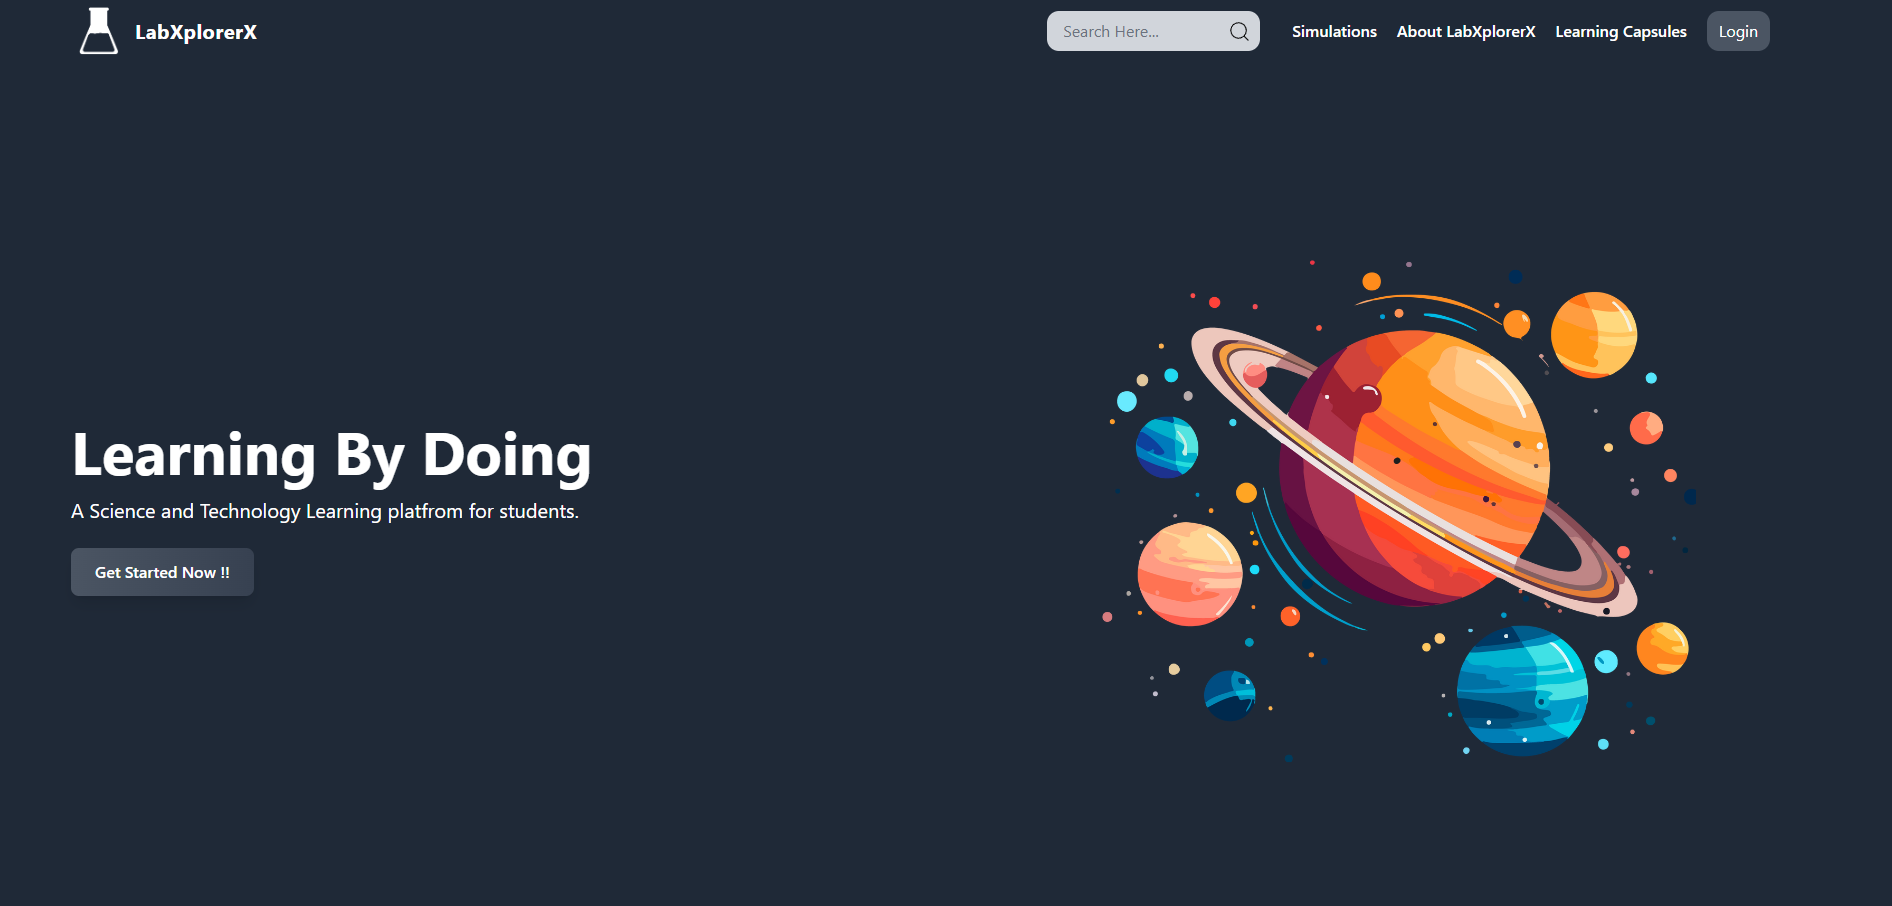
\includegraphics[width = 16cm]{Diagrams/output/home.png}
     \caption{Home Screen}
 \end{figure}

 \begin{figure}[H]
    \centering
     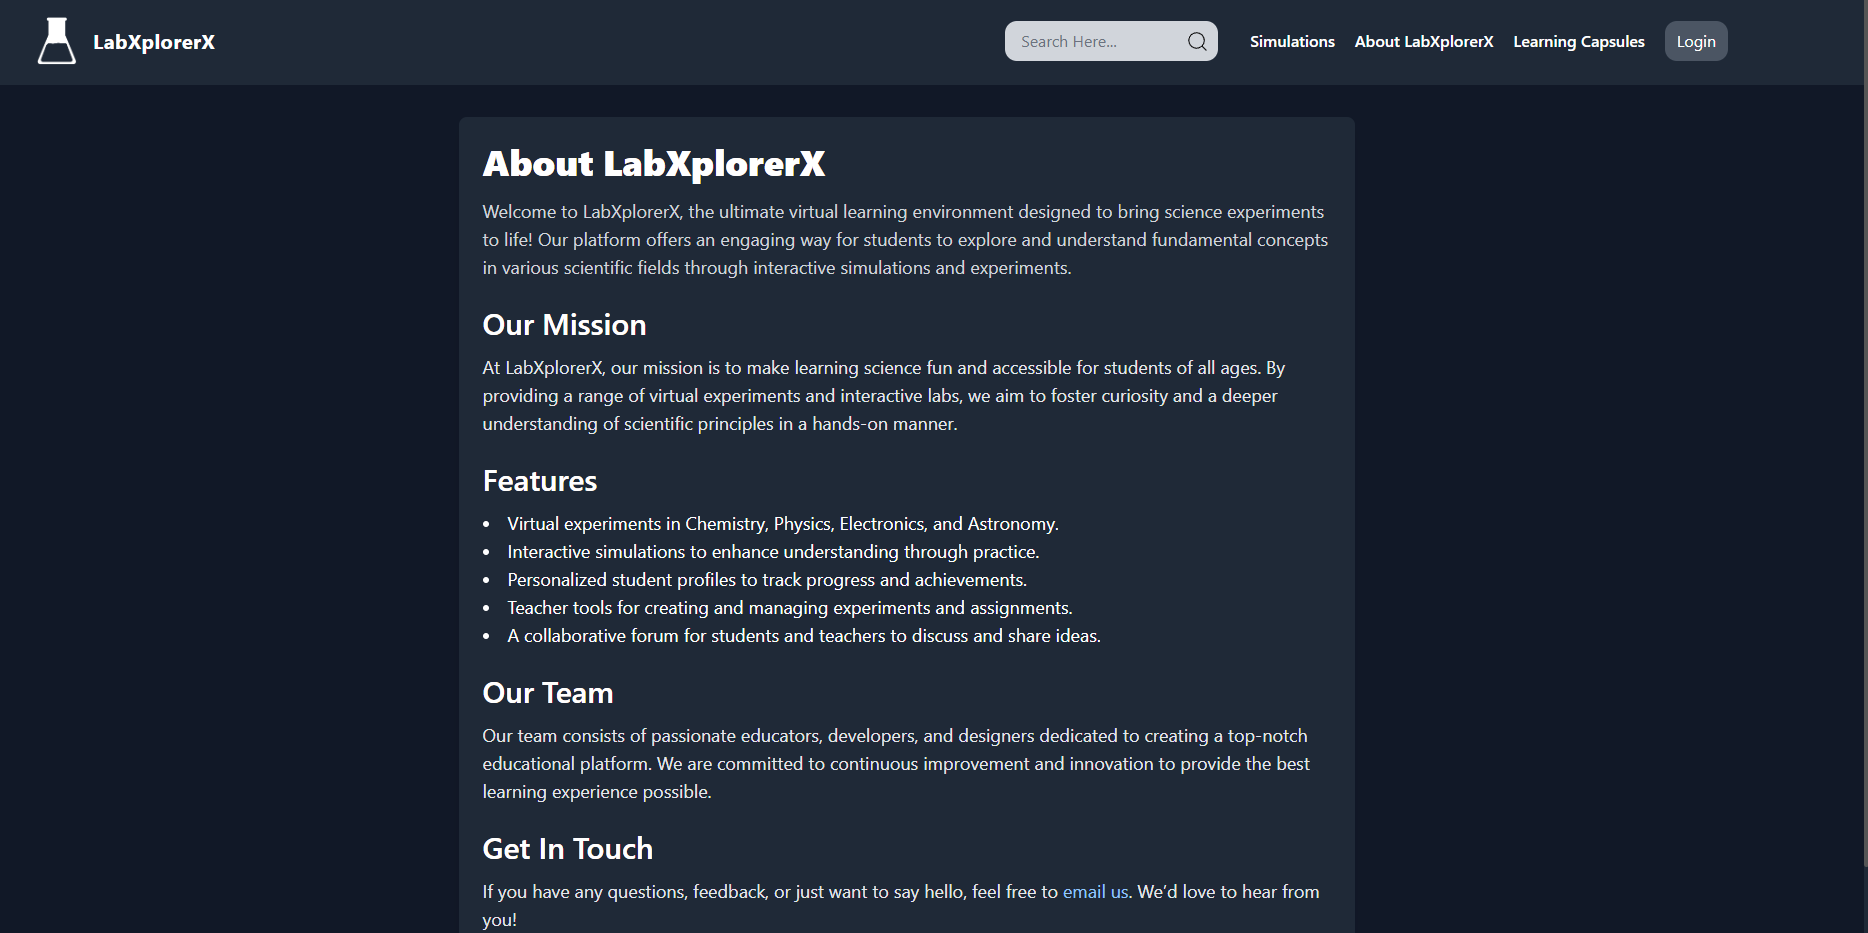
\includegraphics[width = 16cm]{Diagrams/output/about.png}
     \caption{About Page}
 \end{figure}

 \begin{figure}[H]
    \centering
     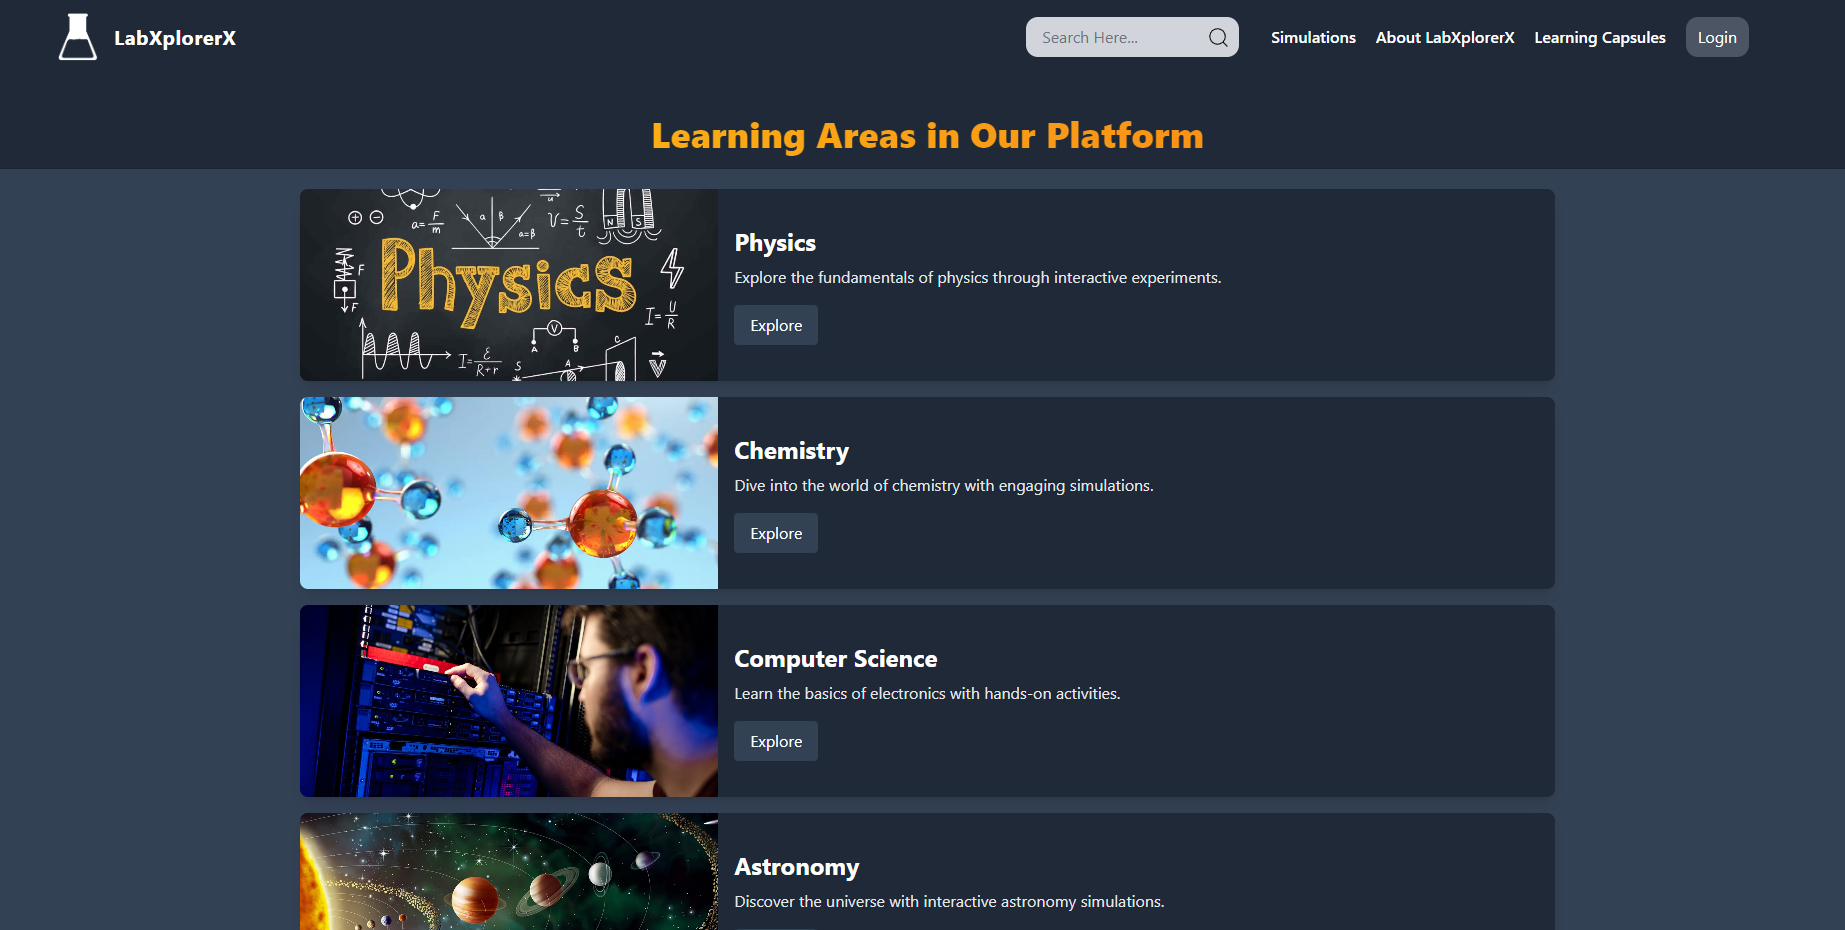
\includegraphics[width = 16cm]{Diagrams/output/learningareas.png}
     \caption{Learning Areas}
 \end{figure}


 \begin{figure}[H]
    \centering
     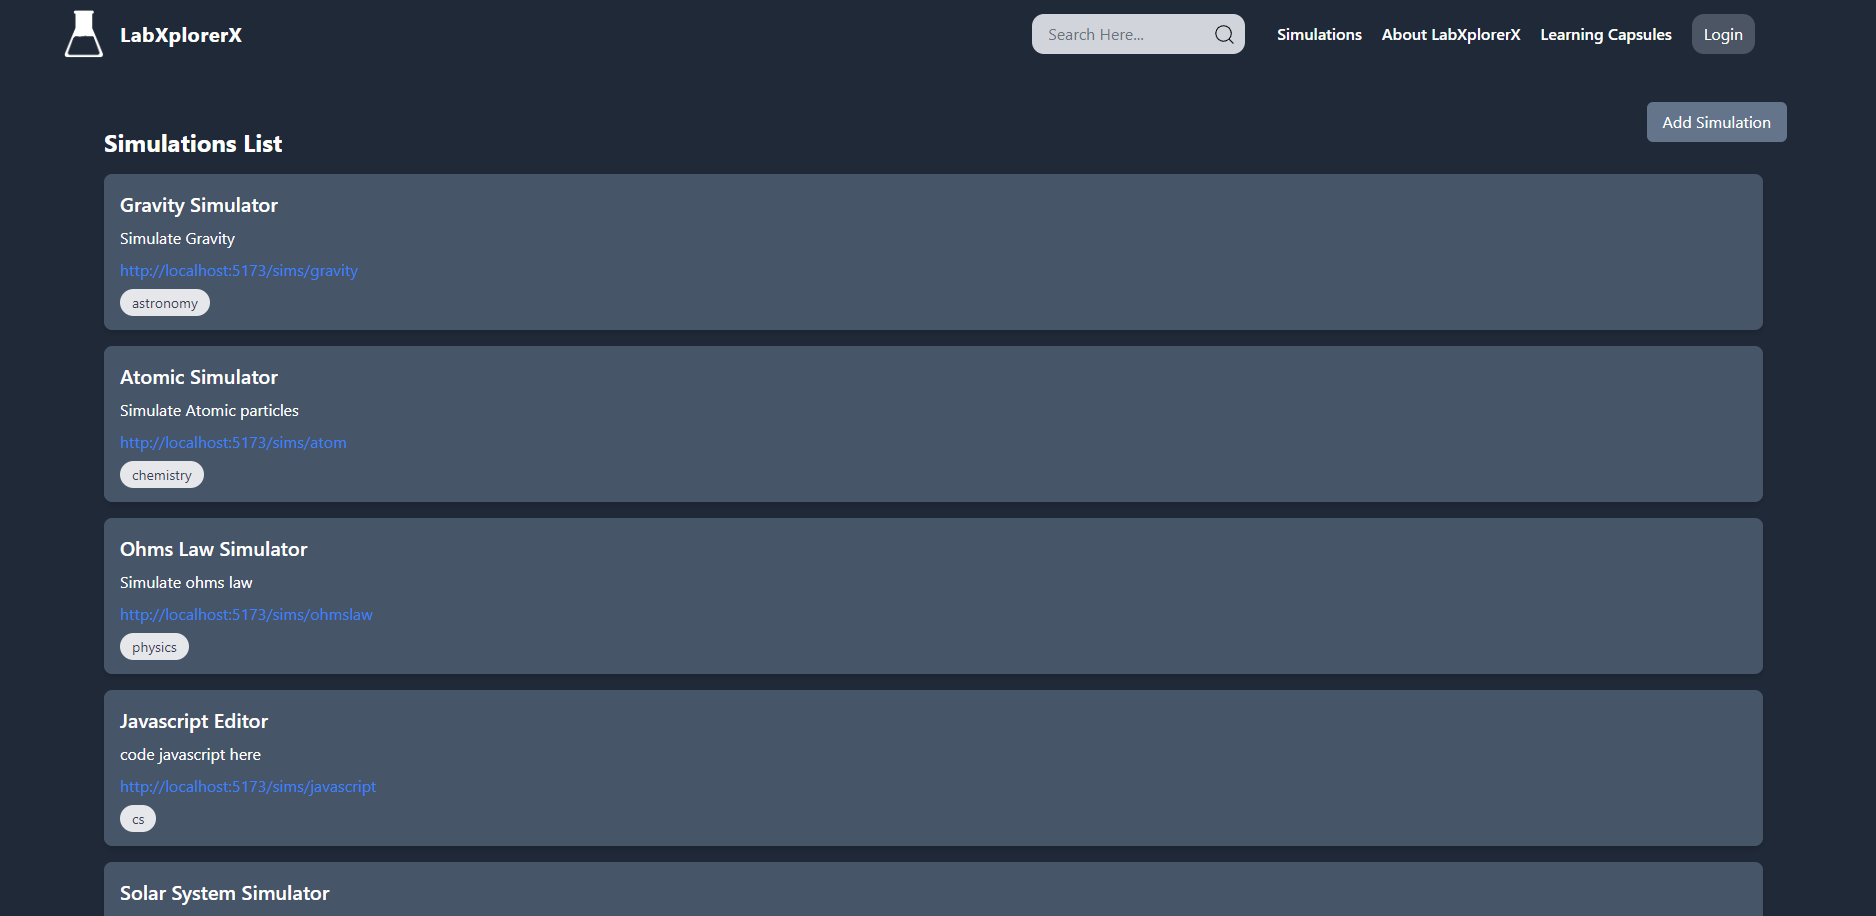
\includegraphics[width = 16cm]{Diagrams/output/simulations.png}
     \caption{Simulations}
 \end{figure}

 \begin{figure}[H]
    \centering
     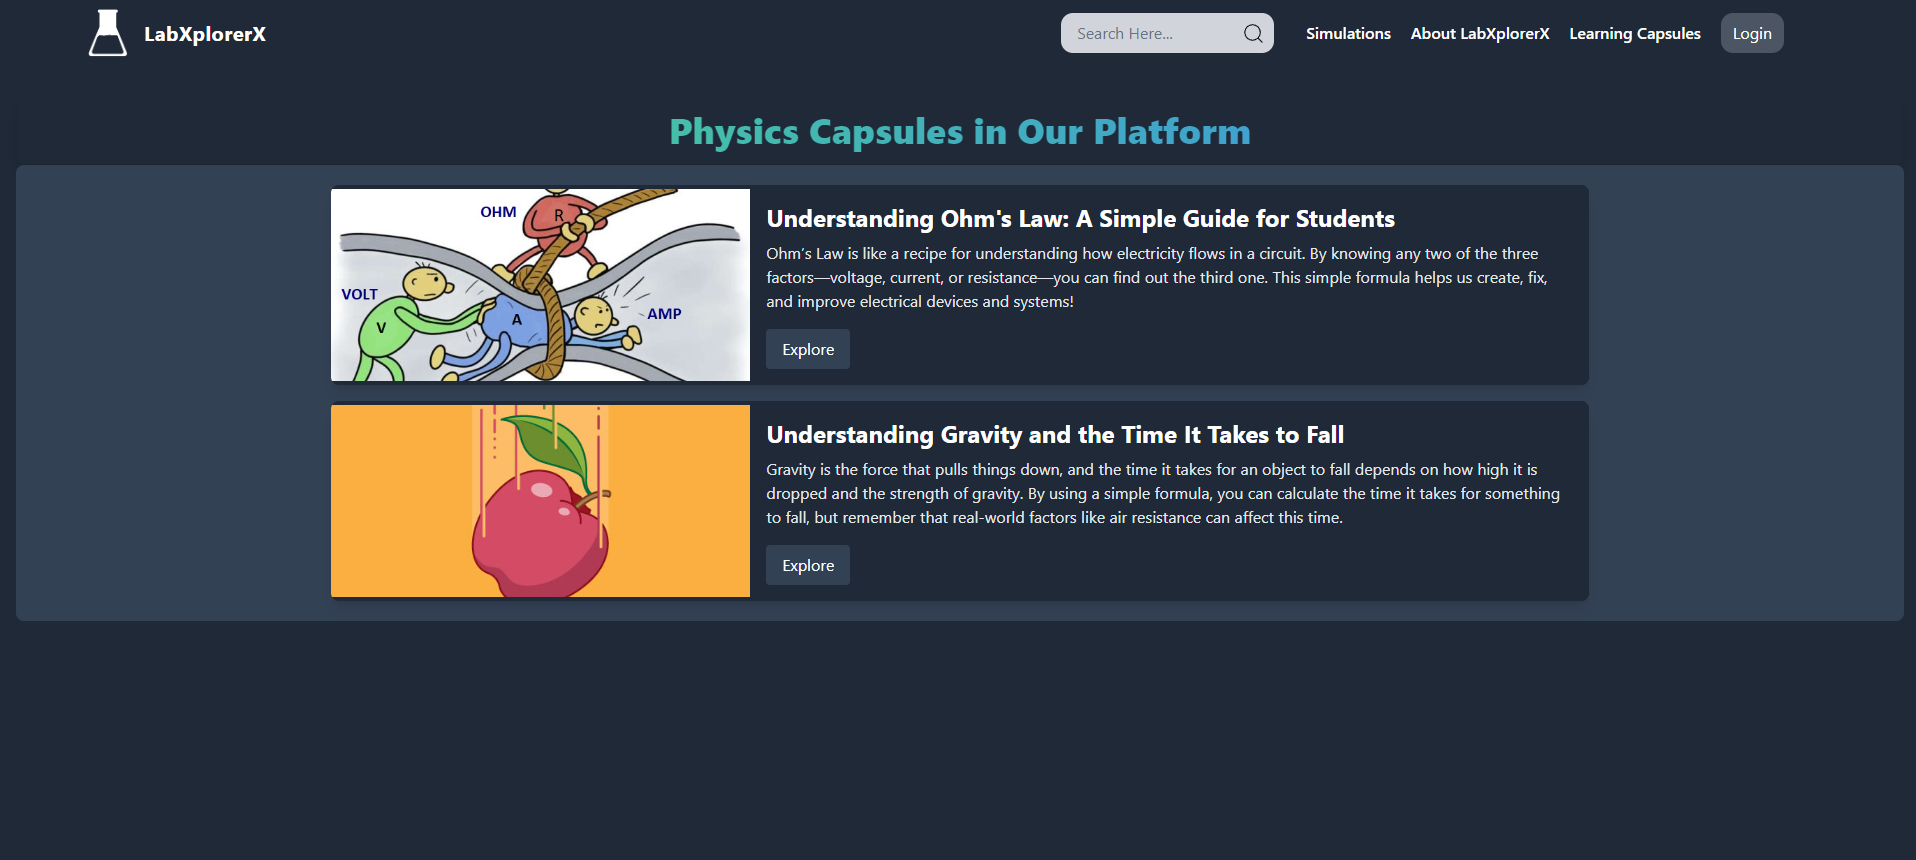
\includegraphics[width = 16cm]{Diagrams/output/capsules.png}
     \caption{Capsules}
 \end{figure}

 \begin{figure}[H]
    \centering
     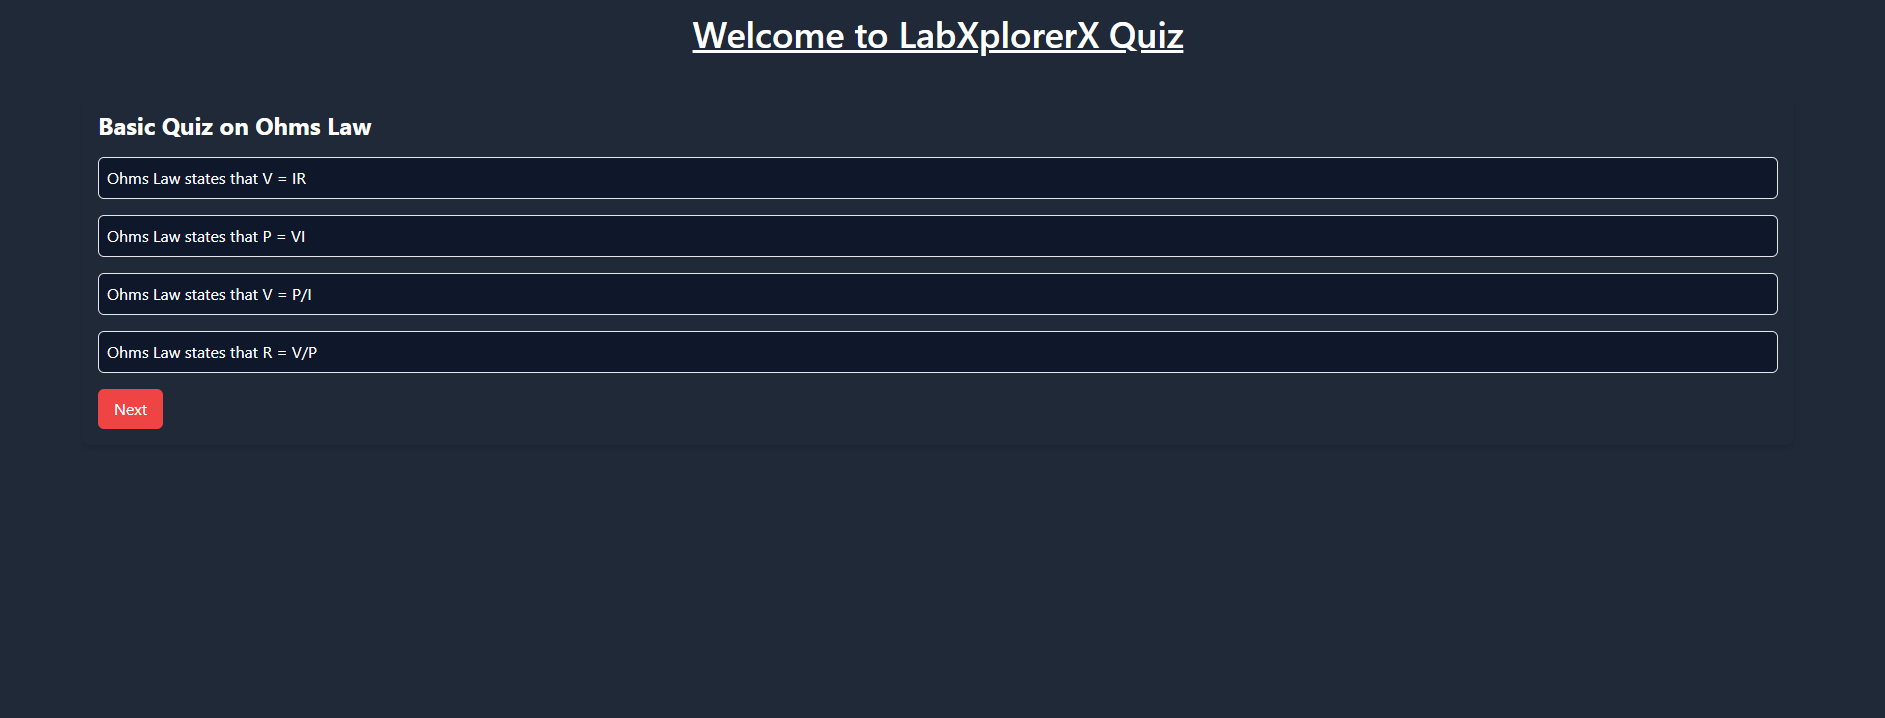
\includegraphics[width = 16cm]{Diagrams/output/quiz.png}
     \caption{Quizzes}
 \end{figure}

 \begin{figure}[H]
    \centering
     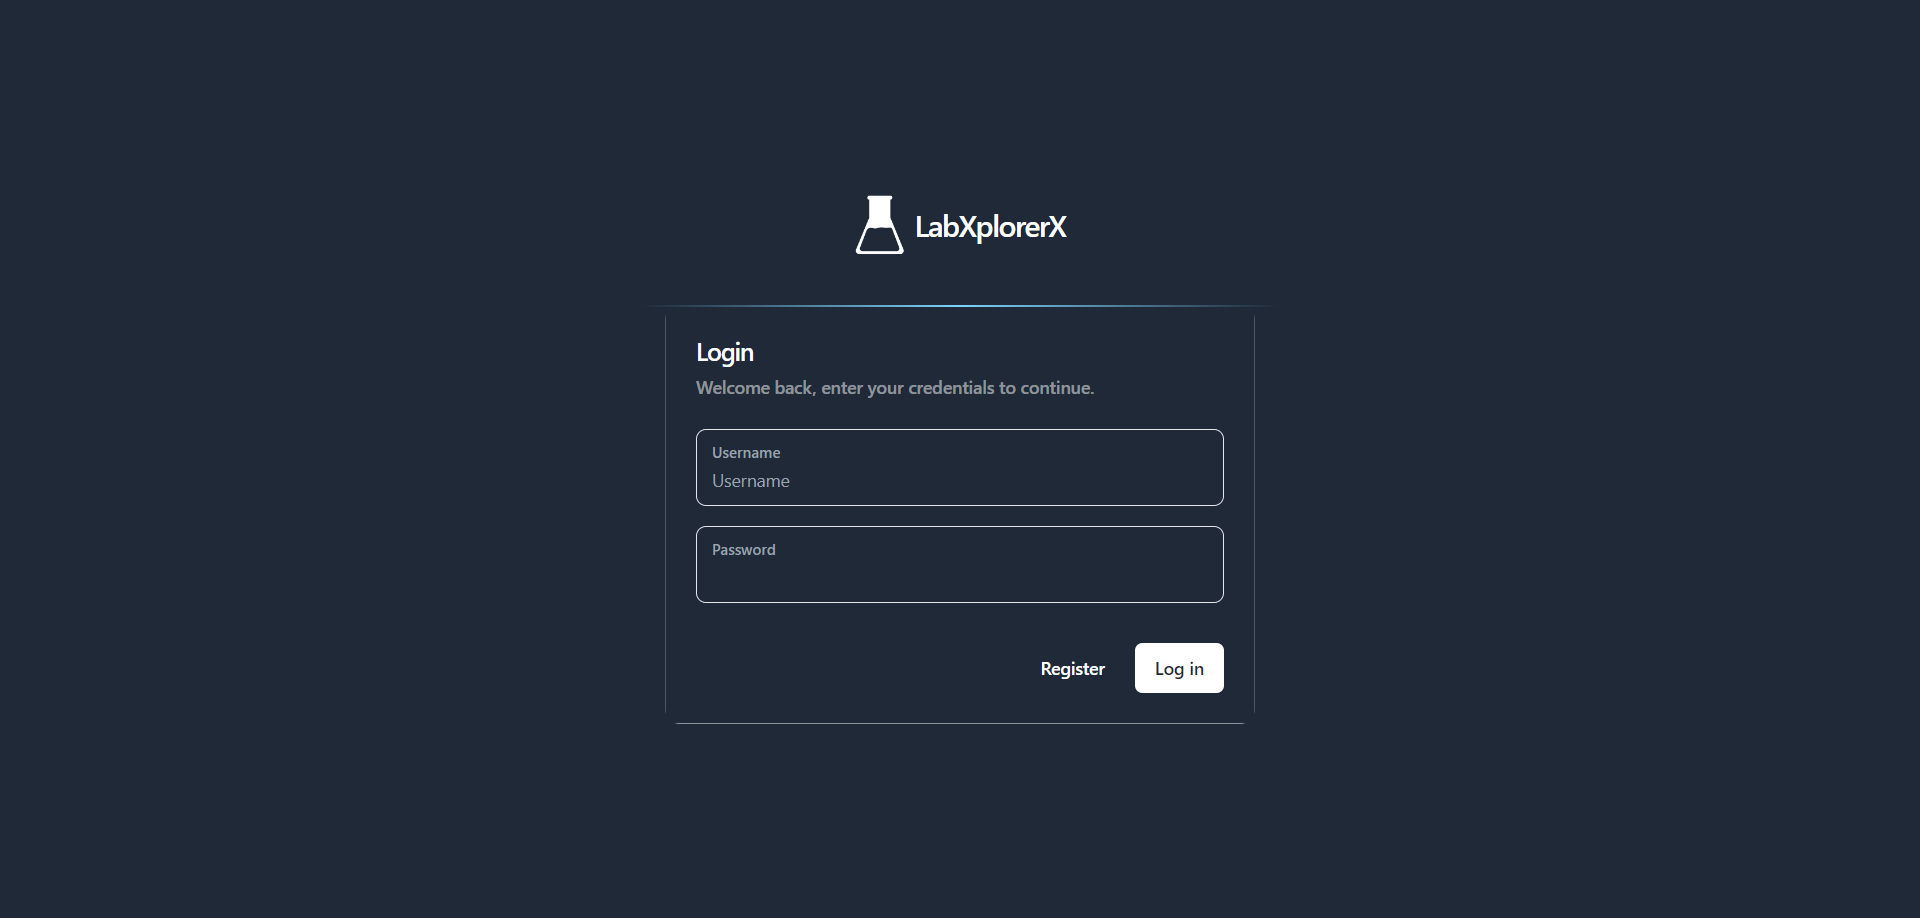
\includegraphics[width = 16cm]{Diagrams/output/login.png}
     \caption{Login}
 \end{figure}

 \begin{figure}[H]
    \centering
     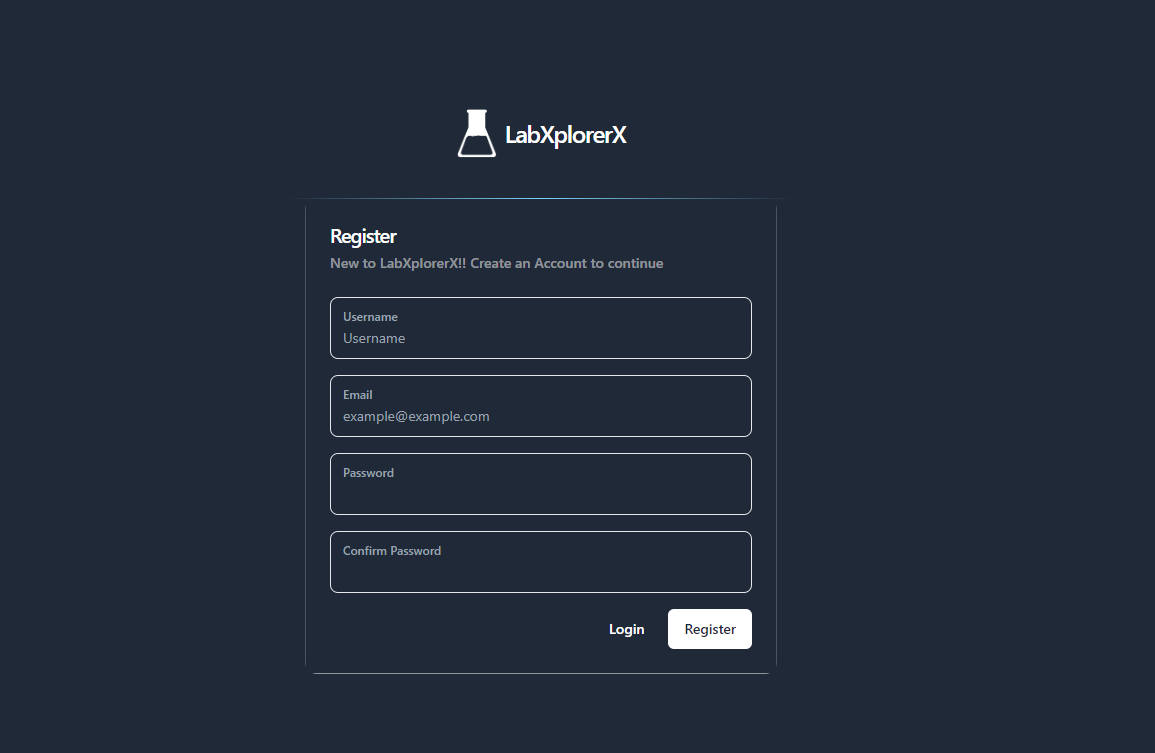
\includegraphics[width = 16cm]{Diagrams/output//register.png}
     \caption{Register}
 \end{figure}

 \begin{figure}[H]
    \centering
     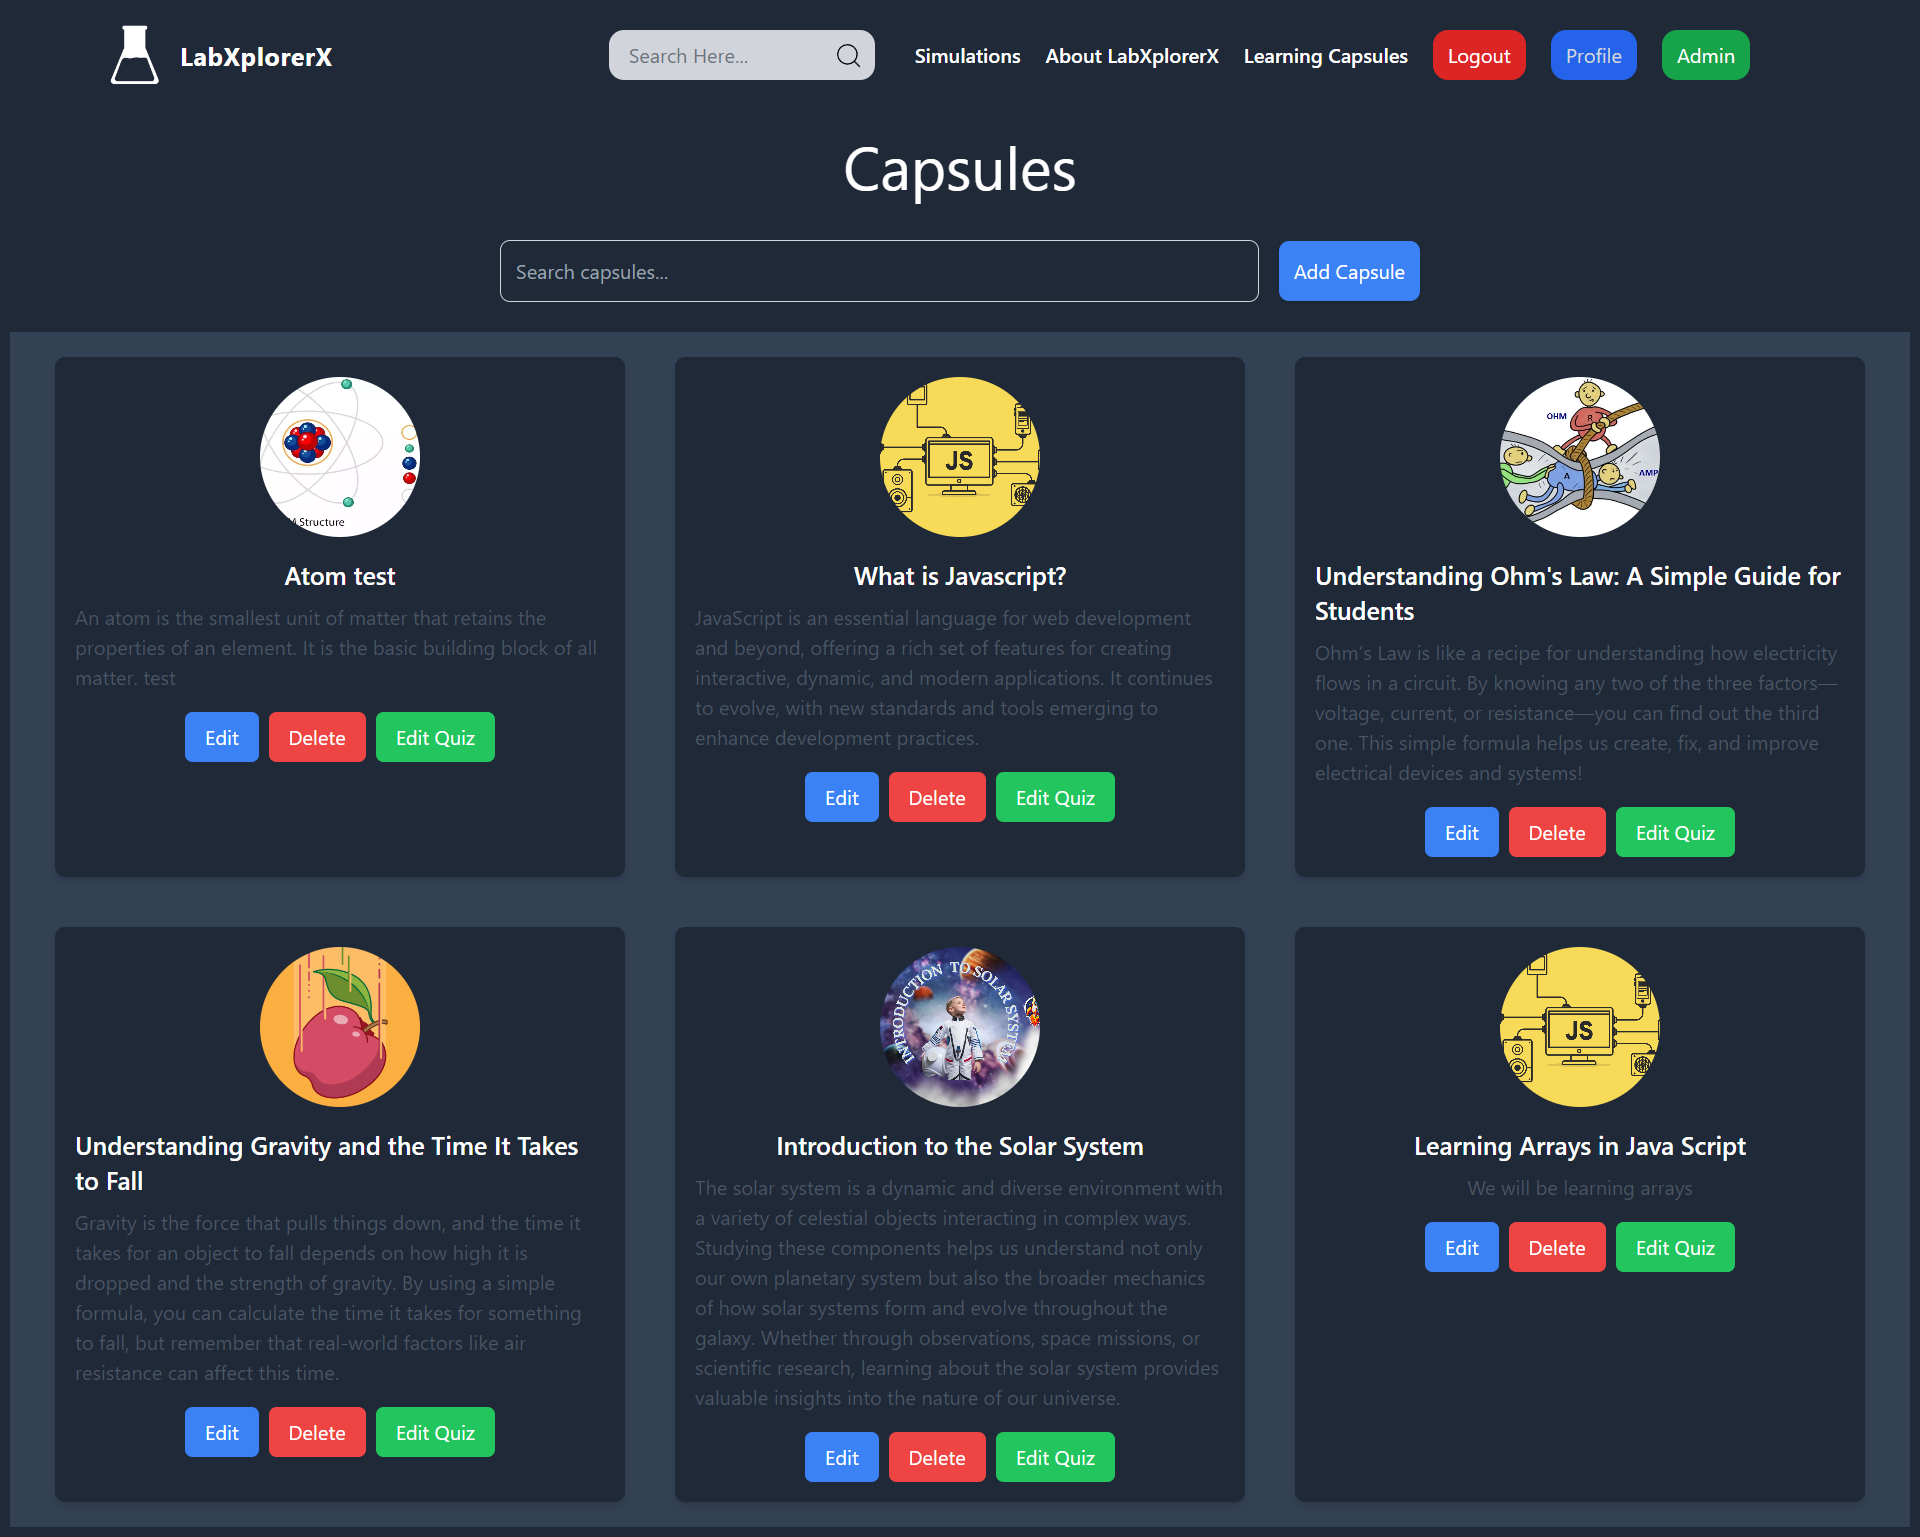
\includegraphics[width = 16cm]{Diagrams/output/admin.png}
     \caption{Admin Panel}
 \end{figure}

 \begin{figure}[H]
    \centering
     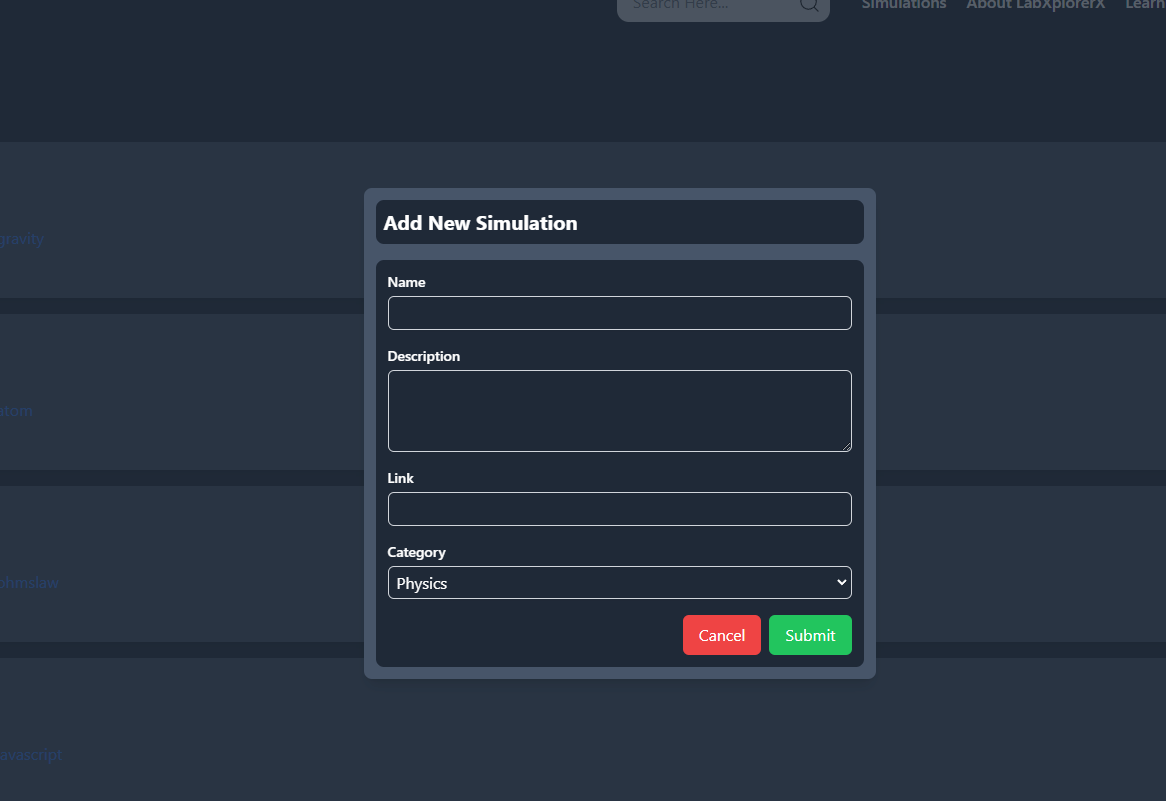
\includegraphics[width = 16cm]{Diagrams/output/addsimulations.png}
     \caption{Add Simulations}
 \end{figure}

 \begin{figure}[H]
    \centering
     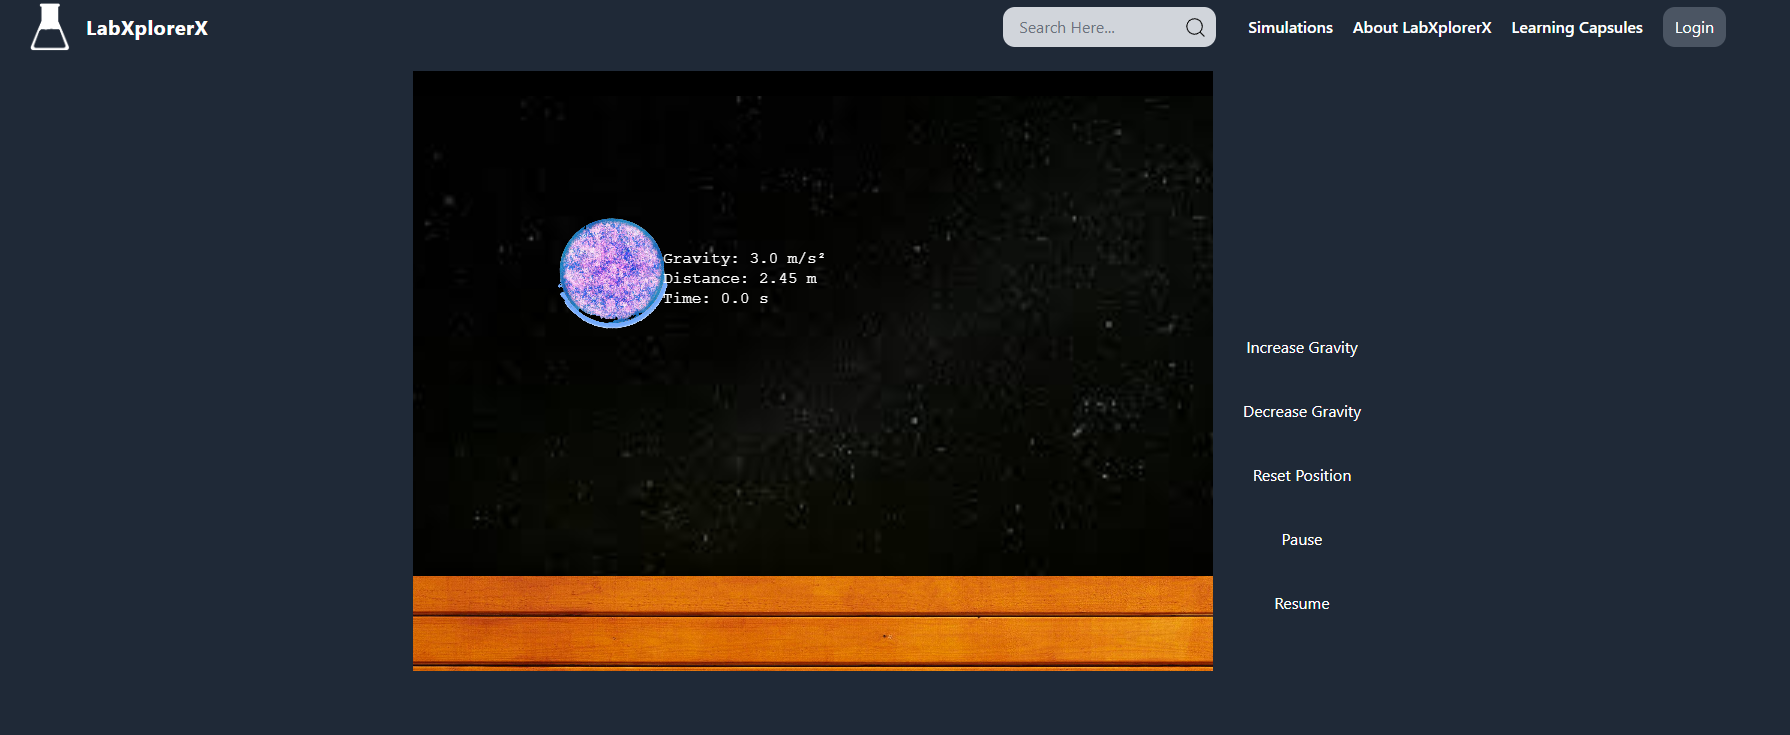
\includegraphics[width = 16cm]{Diagrams/output/gravity.png}
     \caption{Gravity Simulator}
 \end{figure}

 \begin{figure}[H]
    \centering
     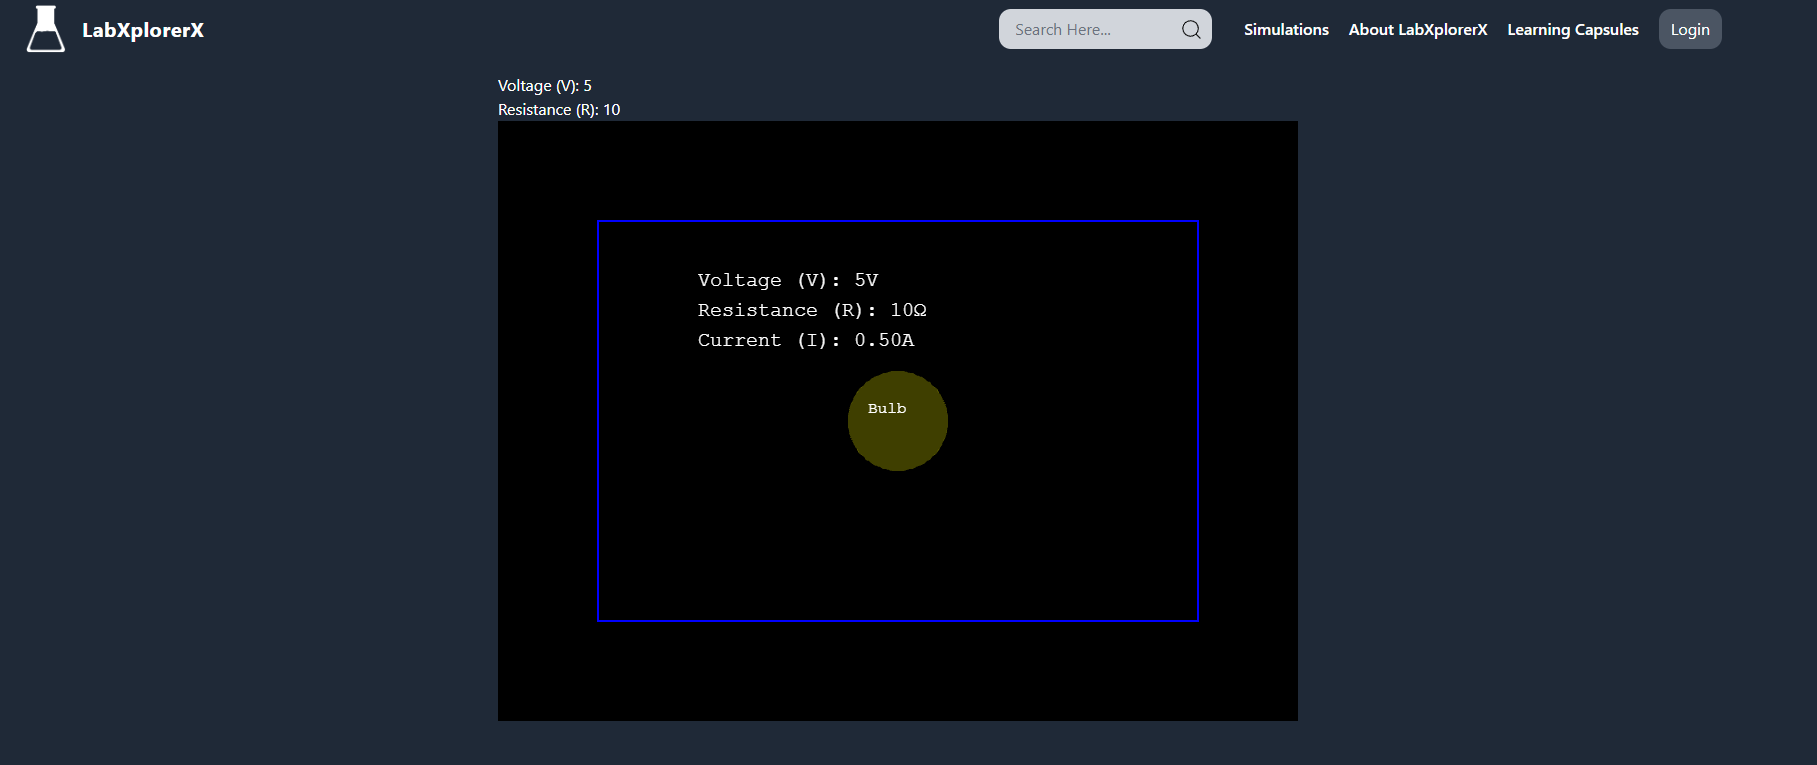
\includegraphics[width = 16cm]{Diagrams/output/ohms.png}
     \caption{Ohms Law Simulator}
 \end{figure}

 \begin{figure}[H]
    \centering
     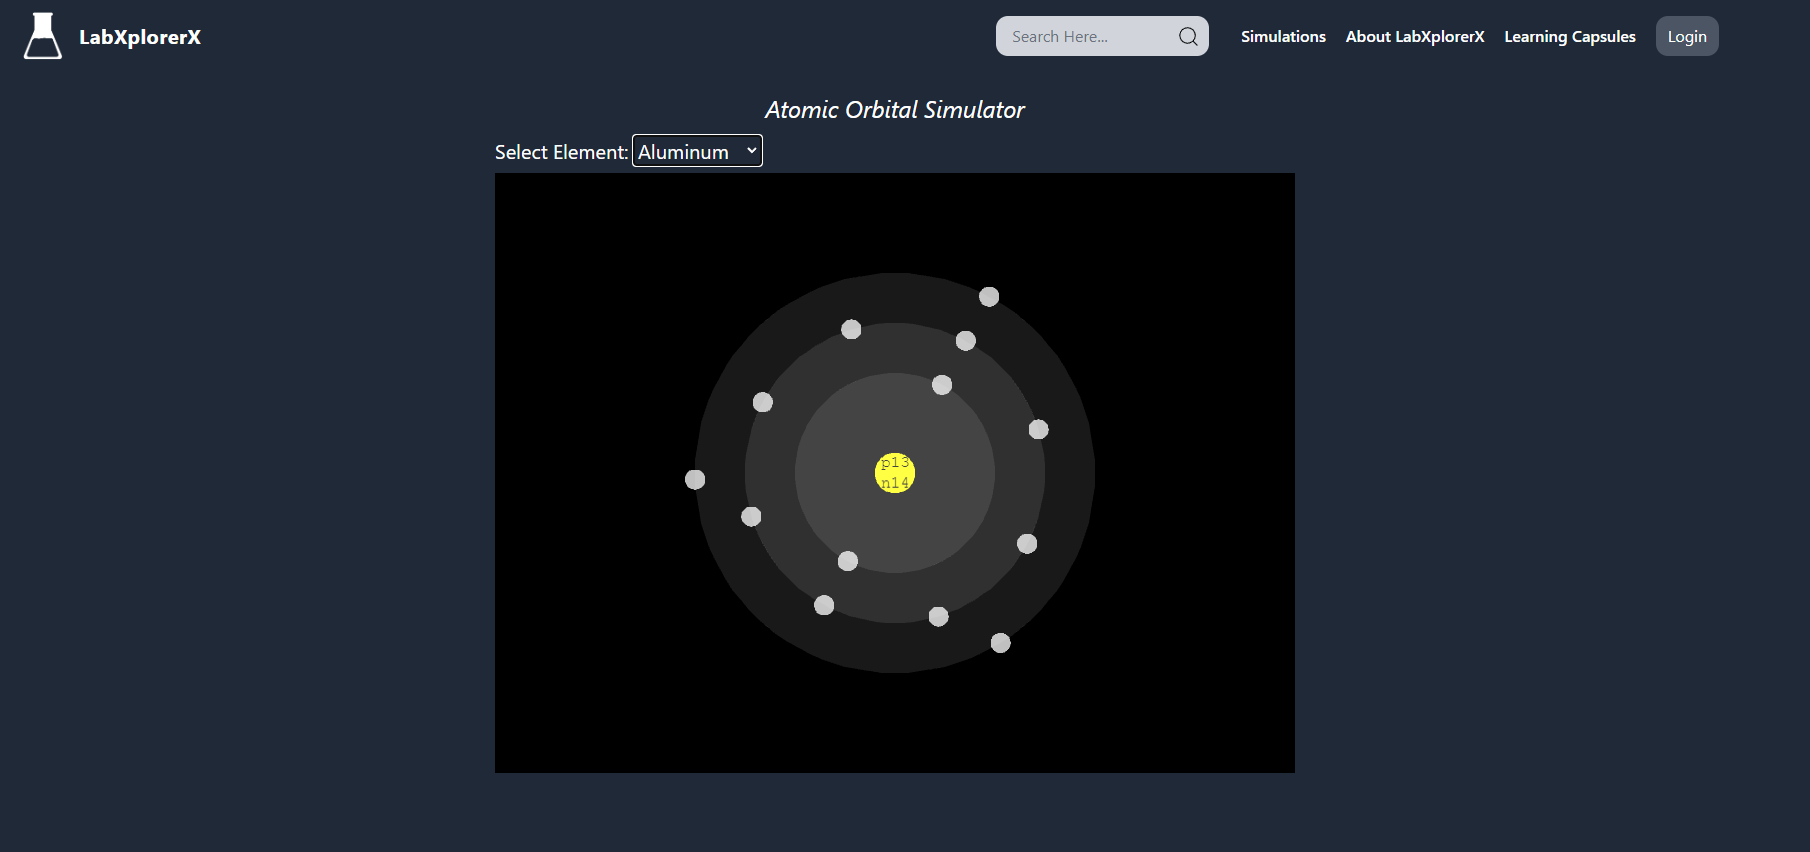
\includegraphics[width = 16cm]{Diagrams/output/atom.png}
     \caption{Atom Simulator}
 \end{figure}

 \begin{figure}[H]
    \centering
     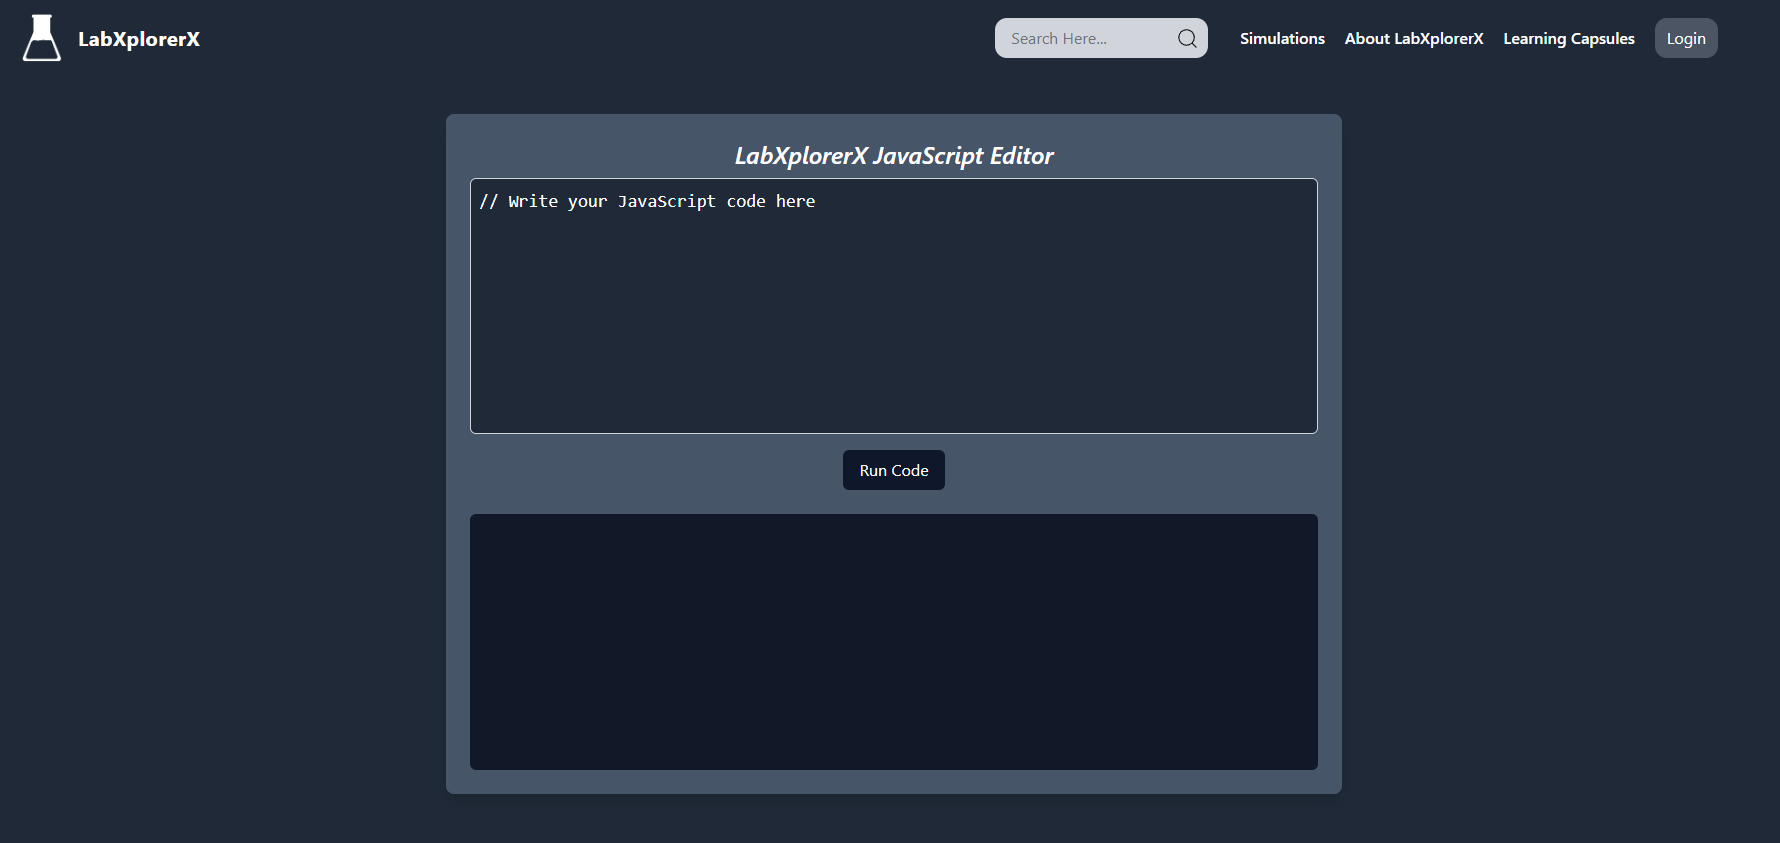
\includegraphics[width = 16cm]{Diagrams/output/js.png}
     \caption{JavaScript Editor}
 \end{figure}
 \begin{figure}[H]
    \centering
     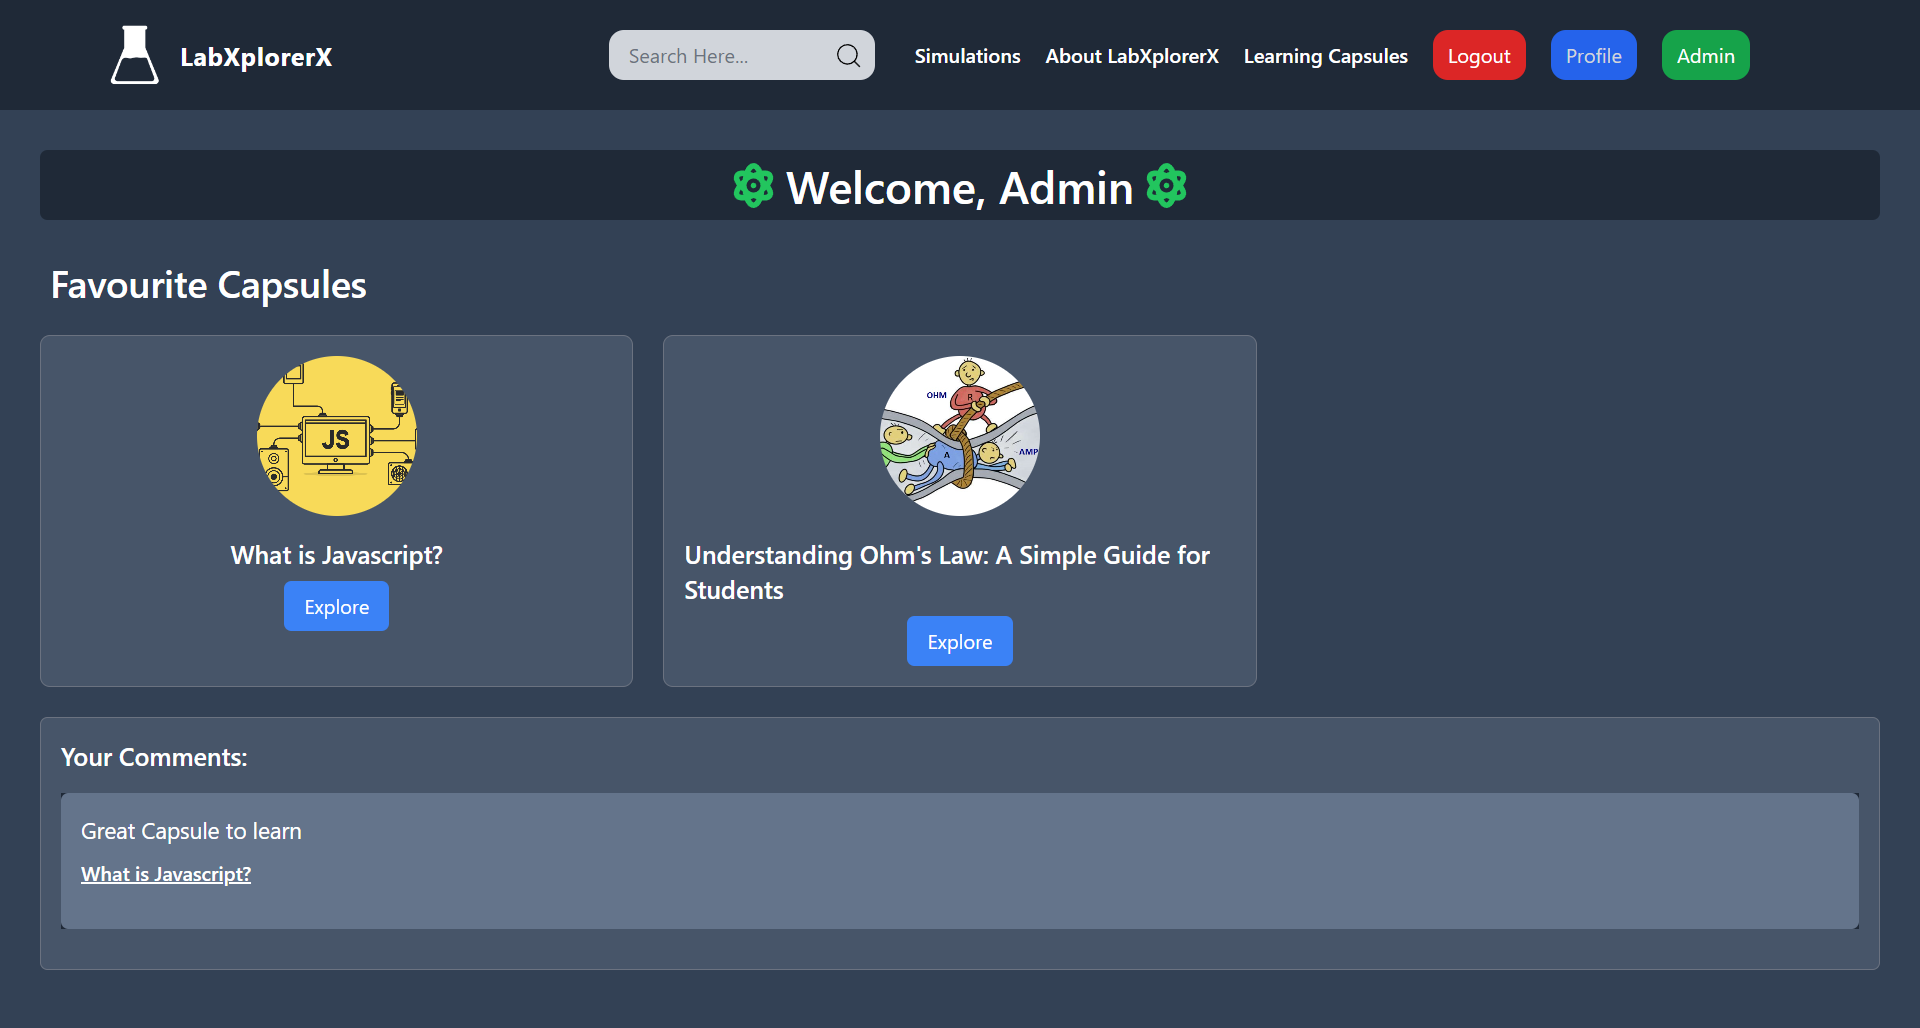
\includegraphics[width = 16cm]{Diagrams/output/profile.png}
     \caption{Profile}
 \end{figure}
 \begin{figure}[H]
    \centering
     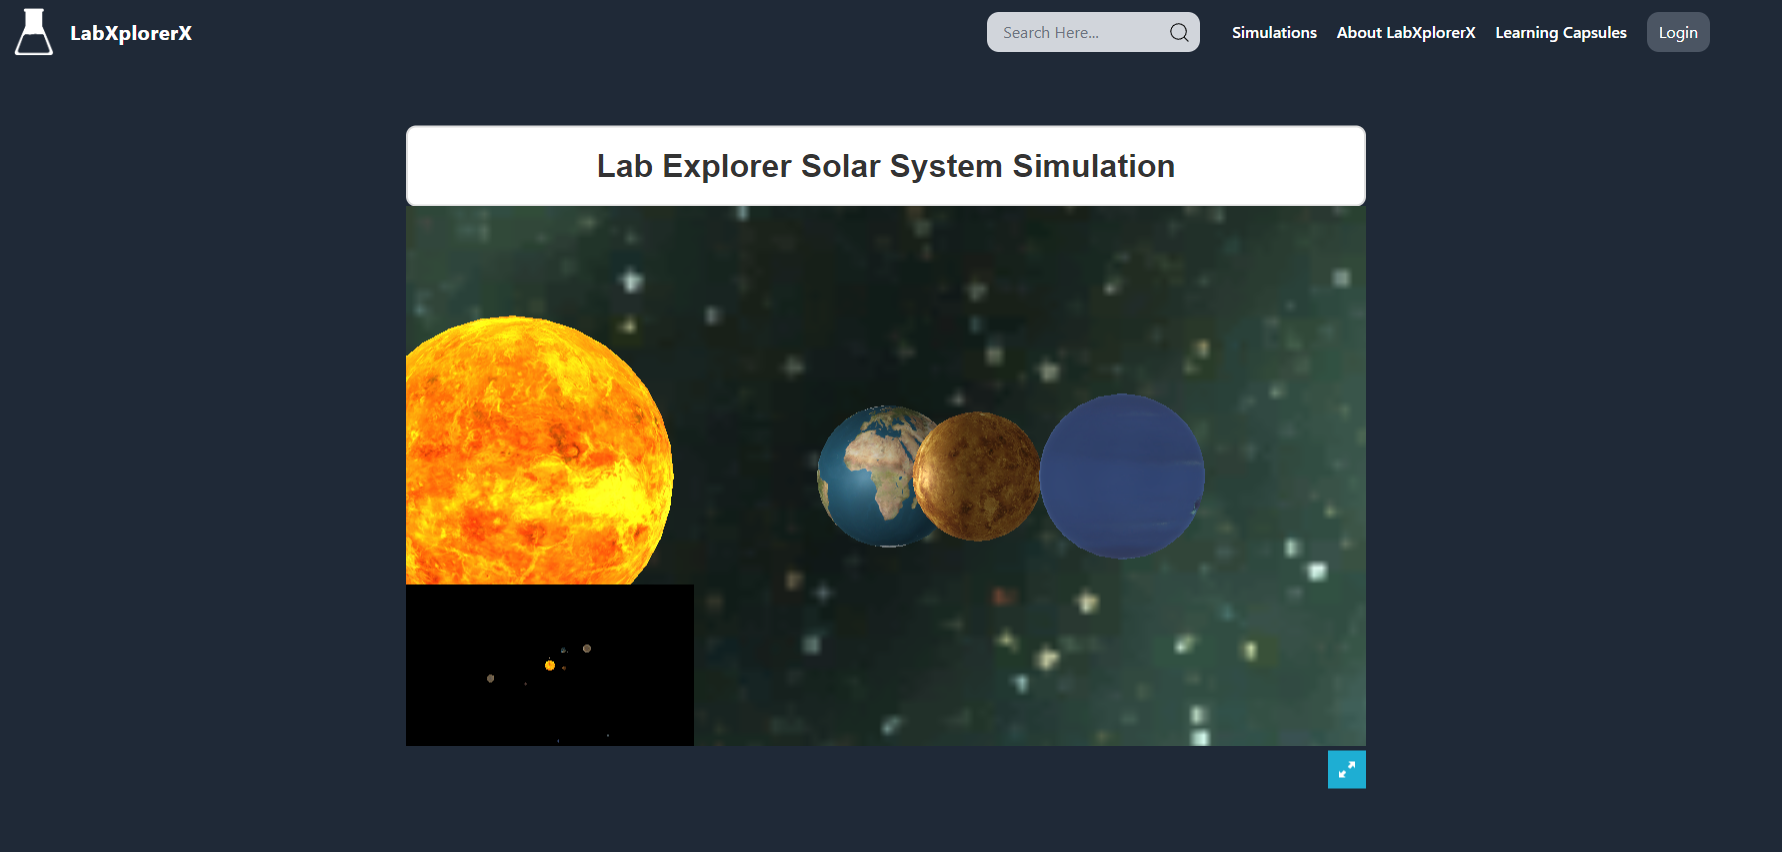
\includegraphics[width = 16cm]{Diagrams/output/solar.png}
     \caption{Solar System Simulator}
 \end{figure}
 \begin{figure}[H]
    \centering
     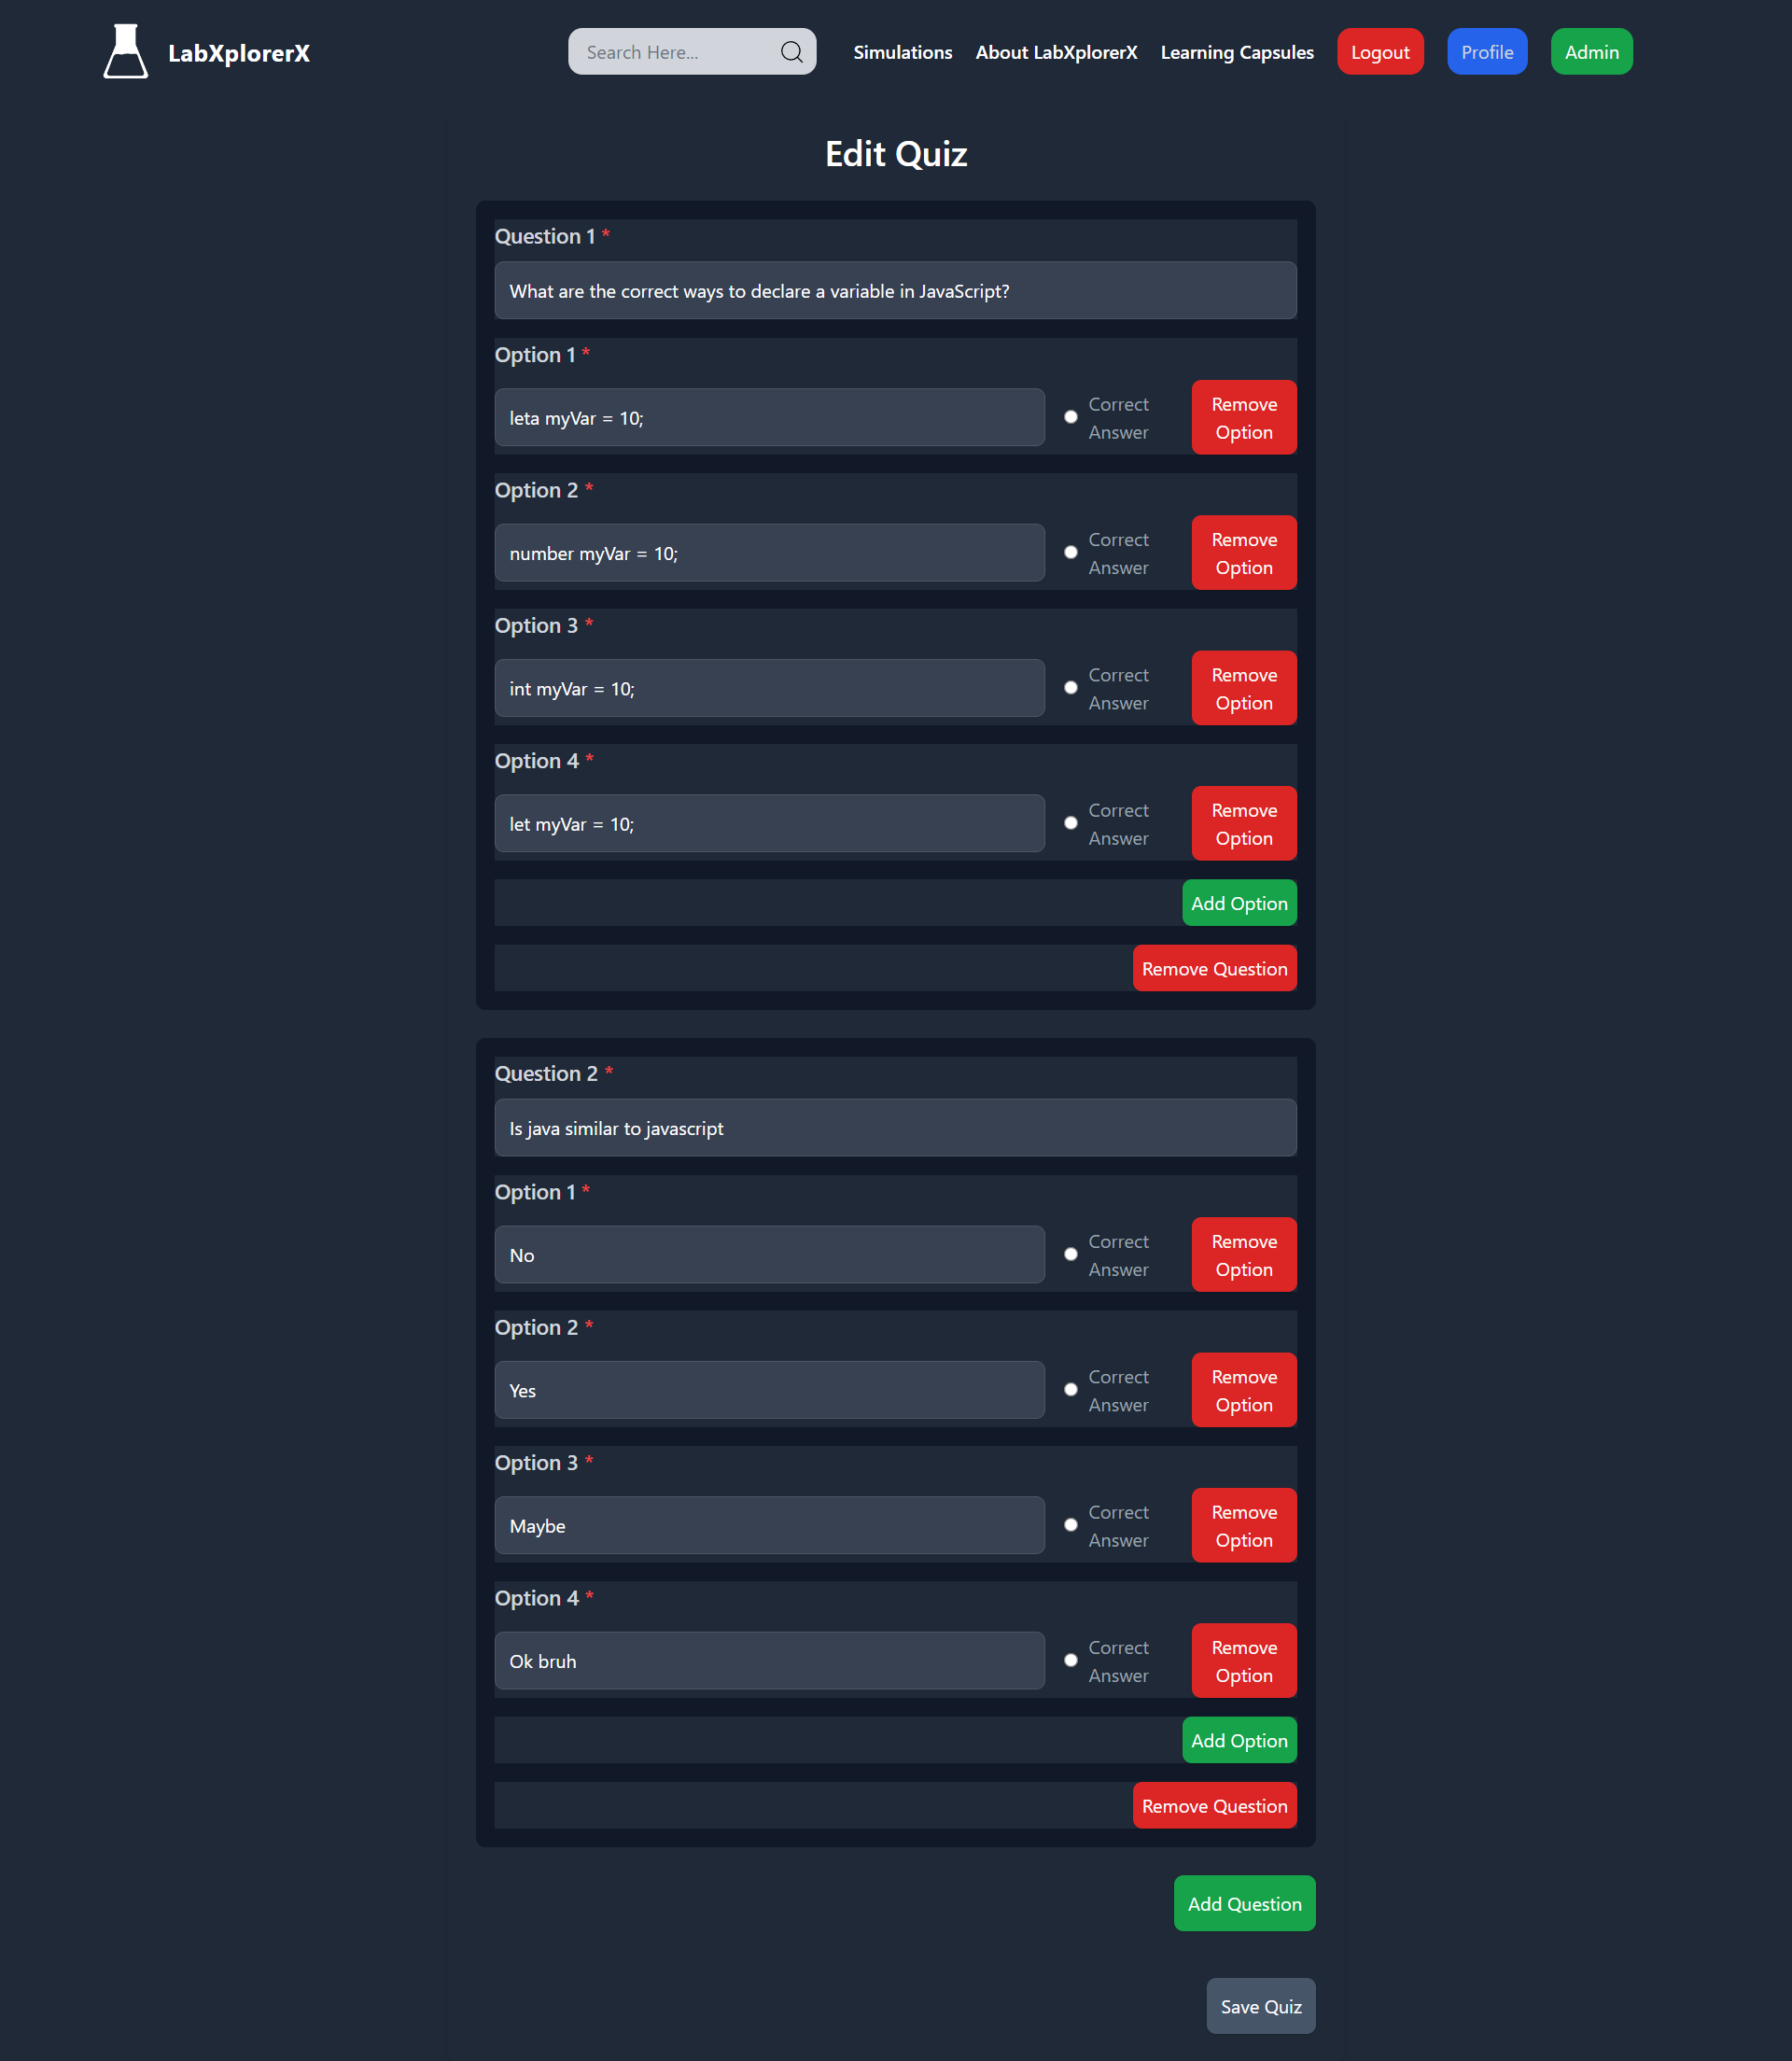
\includegraphics[width = 16cm]{Diagrams/output/edit_quiz.png}
     \caption{CRUD Quizes}
 \end{figure}
 \begin{figure}[H]
    \centering
     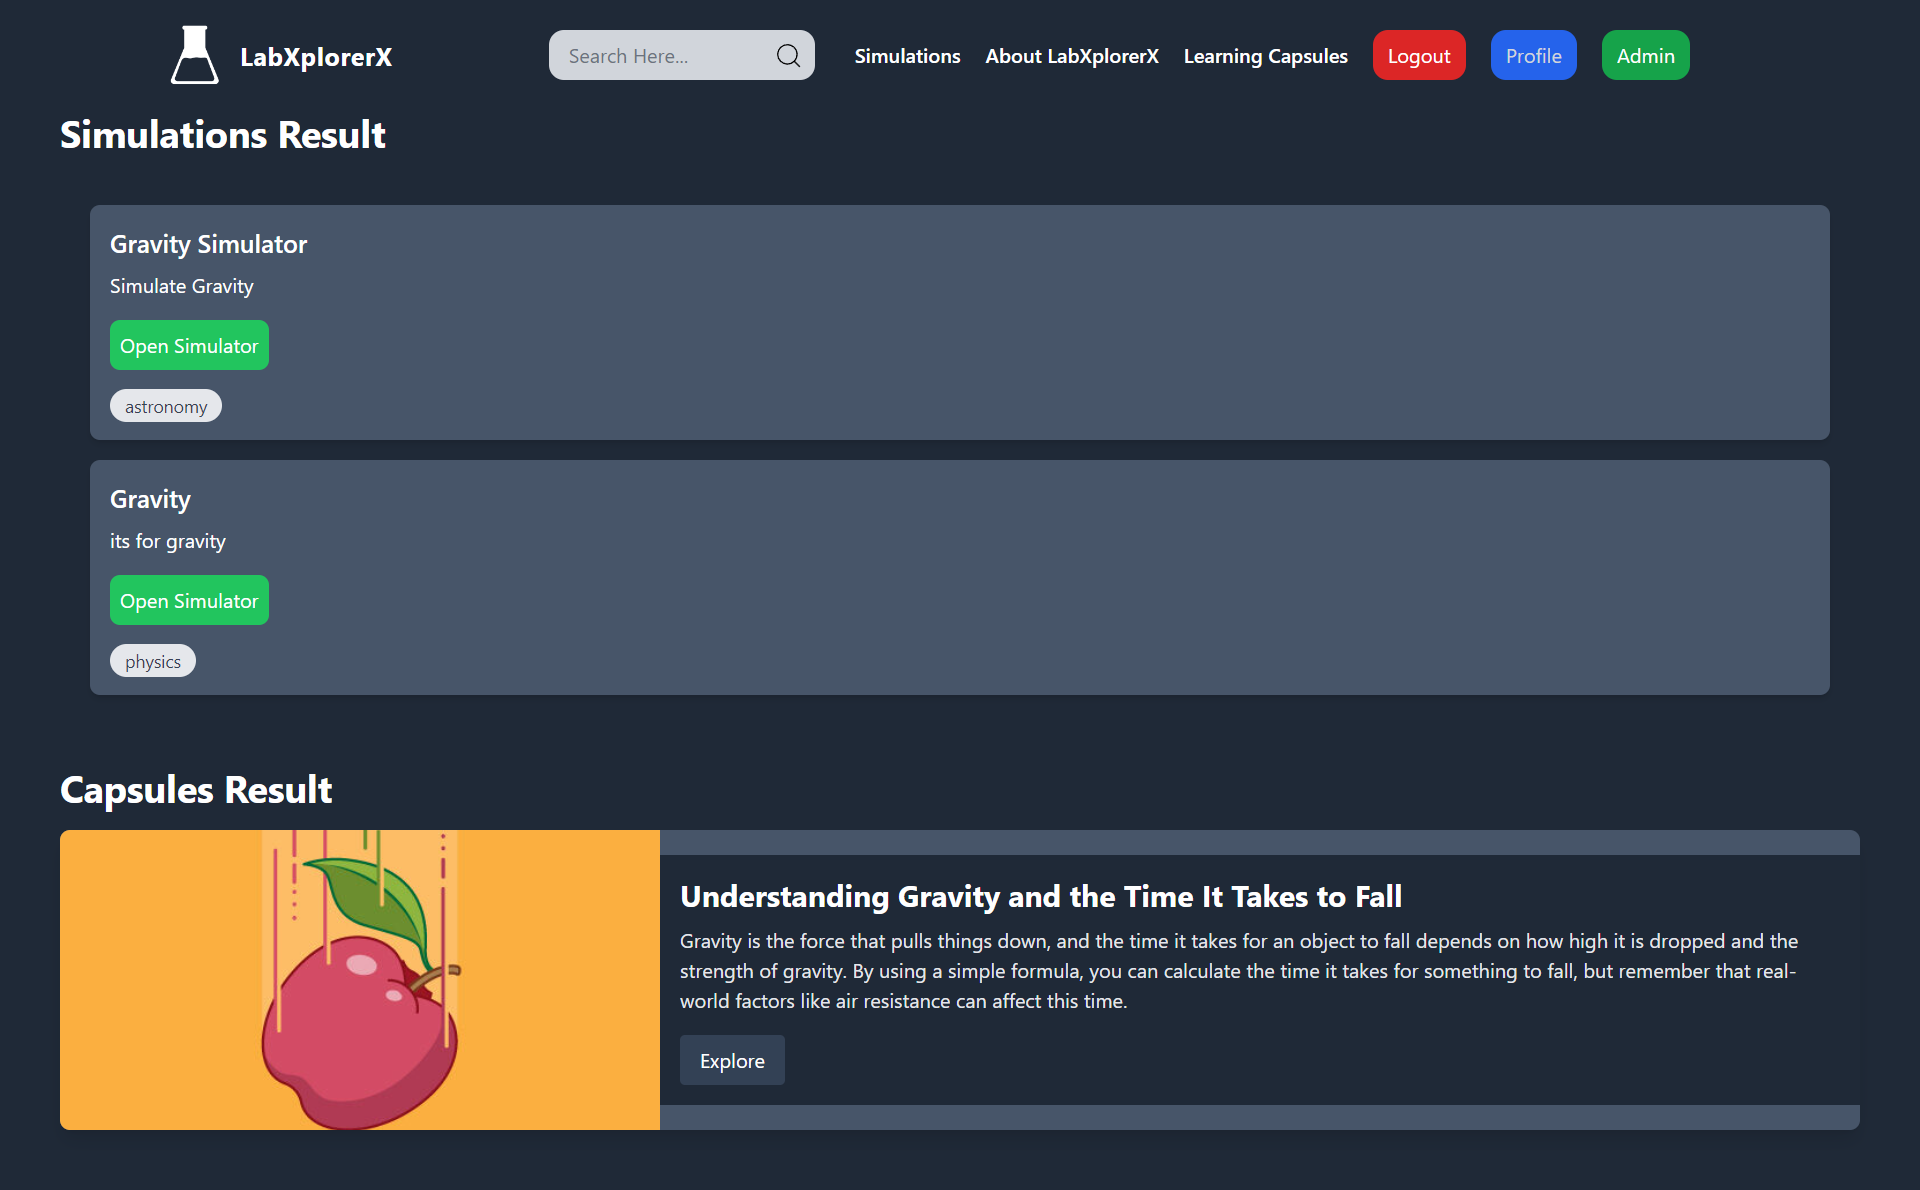
\includegraphics[width = 16cm]{Diagrams/output/search_results.png}
     \caption{Search Results}
 \end{figure}
 \begin{figure}[H]
    \centering
     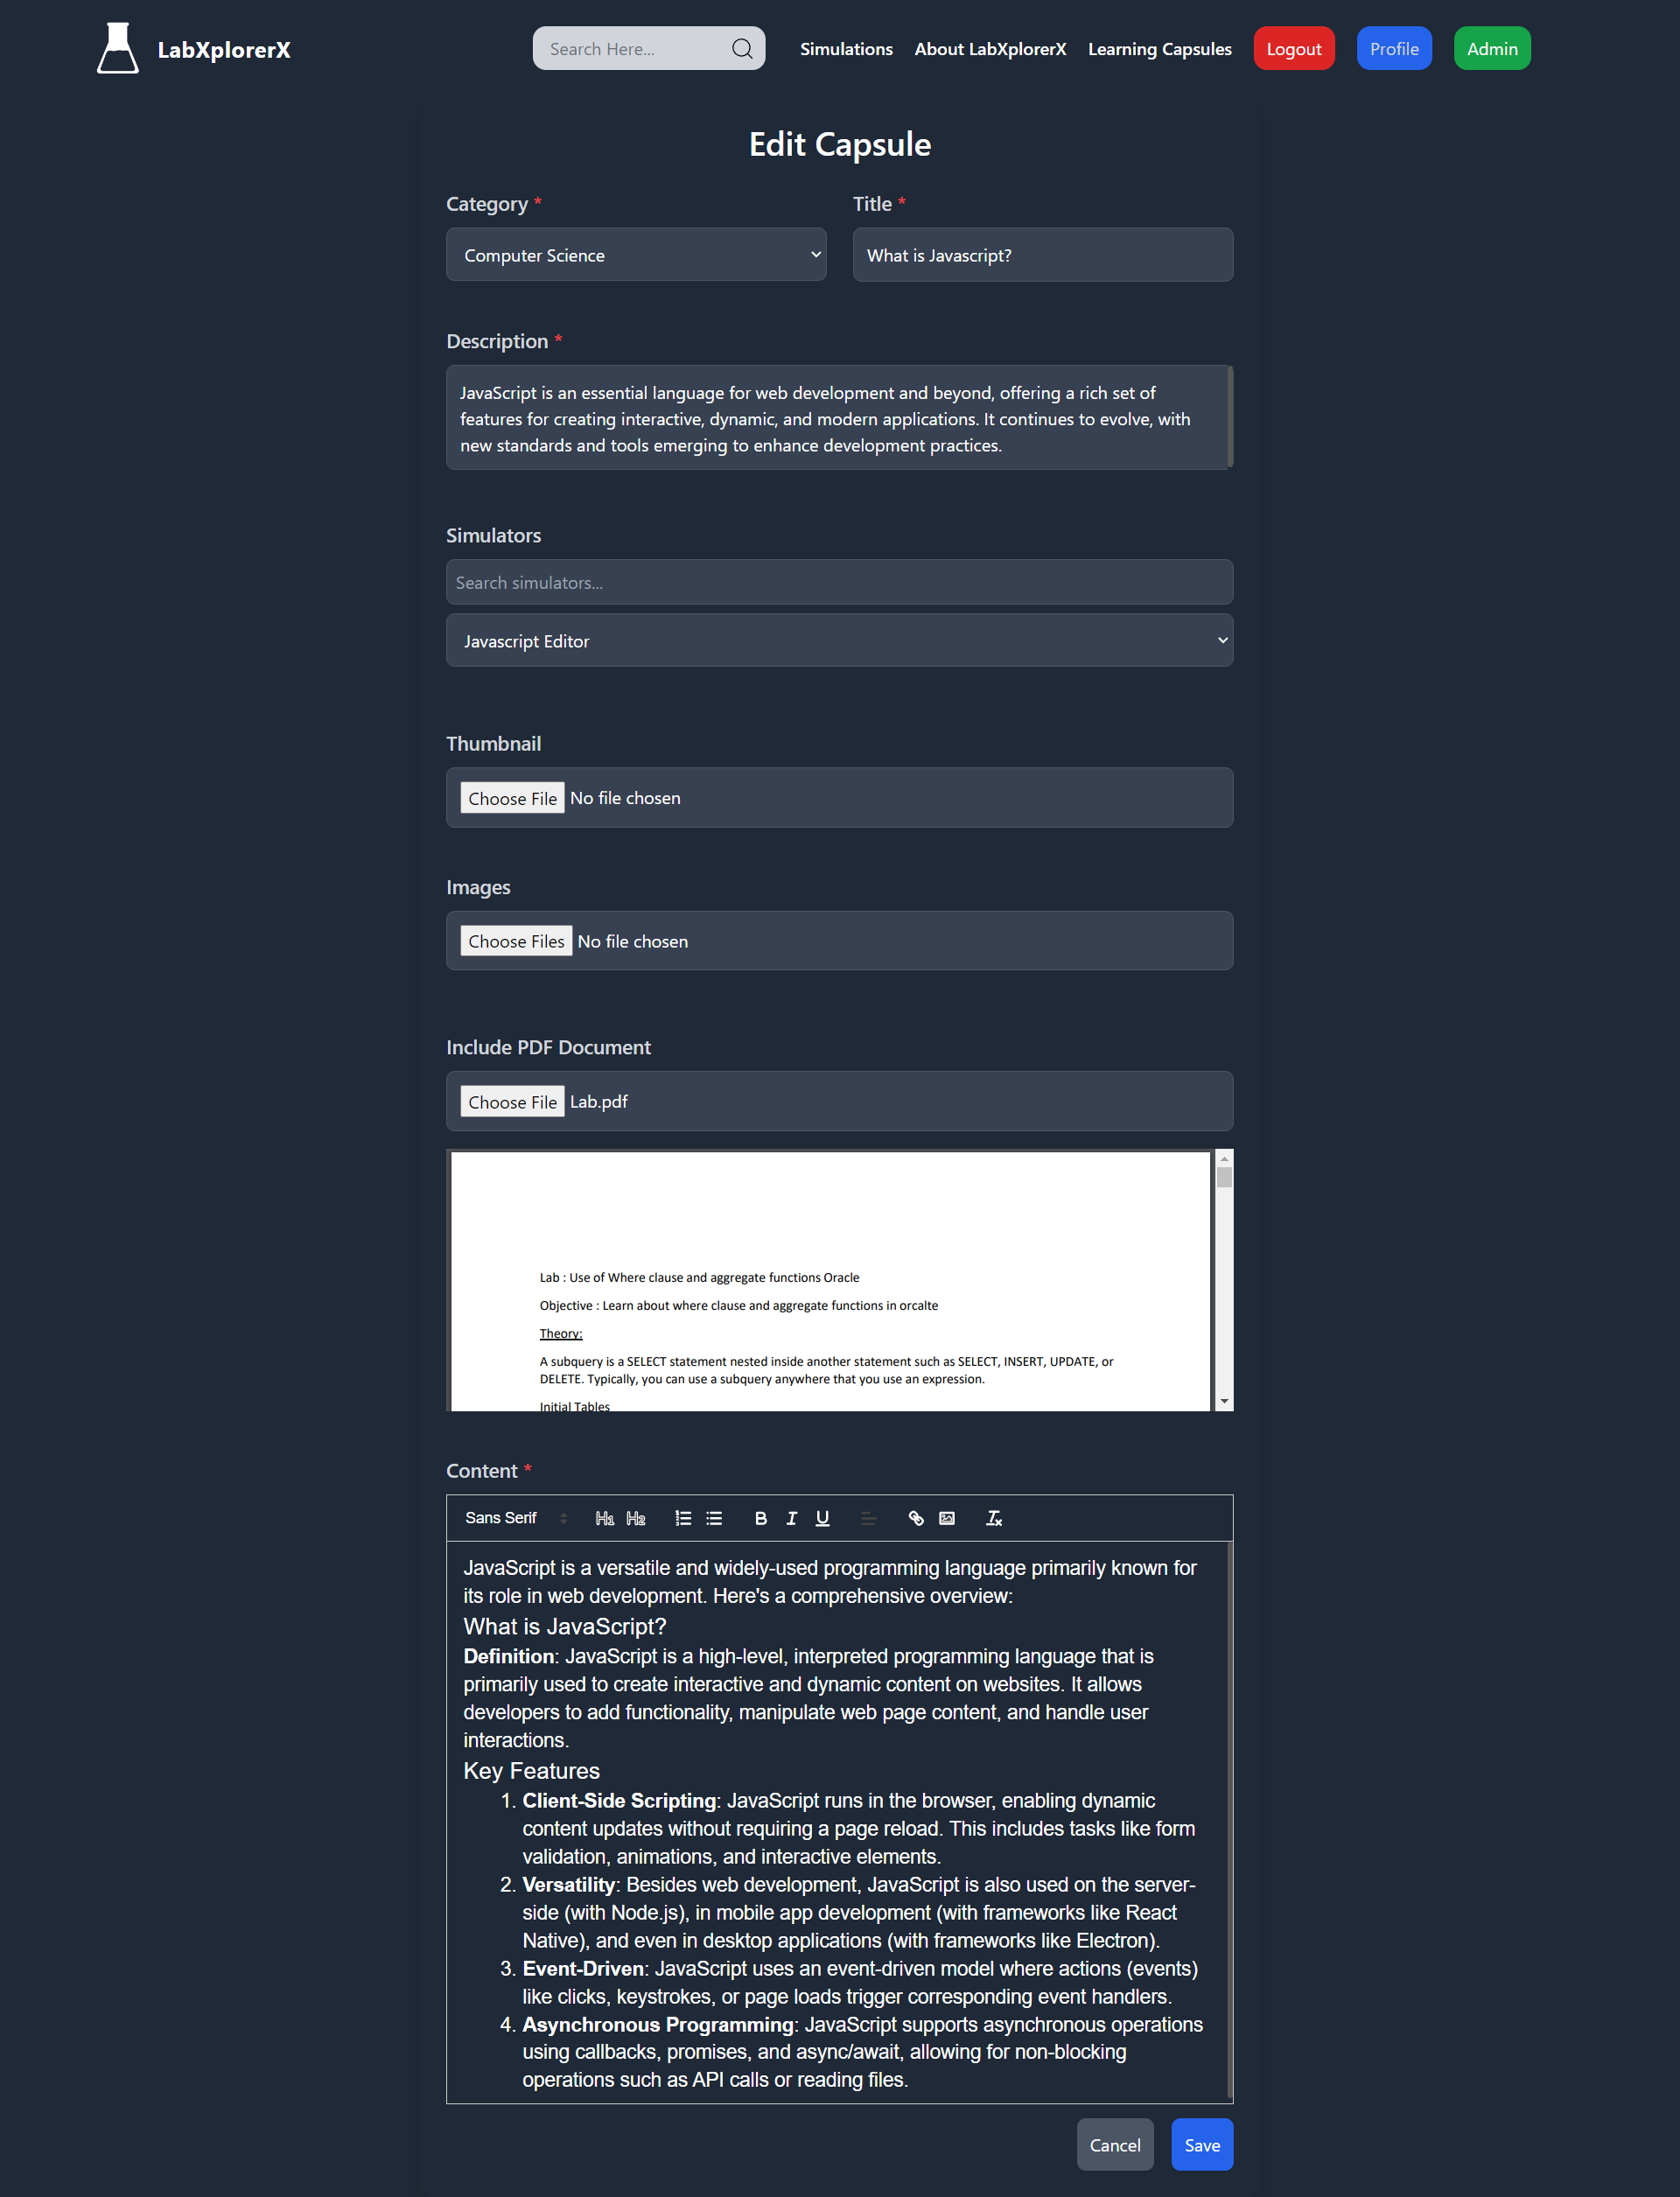
\includegraphics[width = 16cm]{Diagrams/output/edit_capsule.png}
     \caption{Edit Capsule}
 \end{figure}
 \begin{figure}[H]
    \centering
     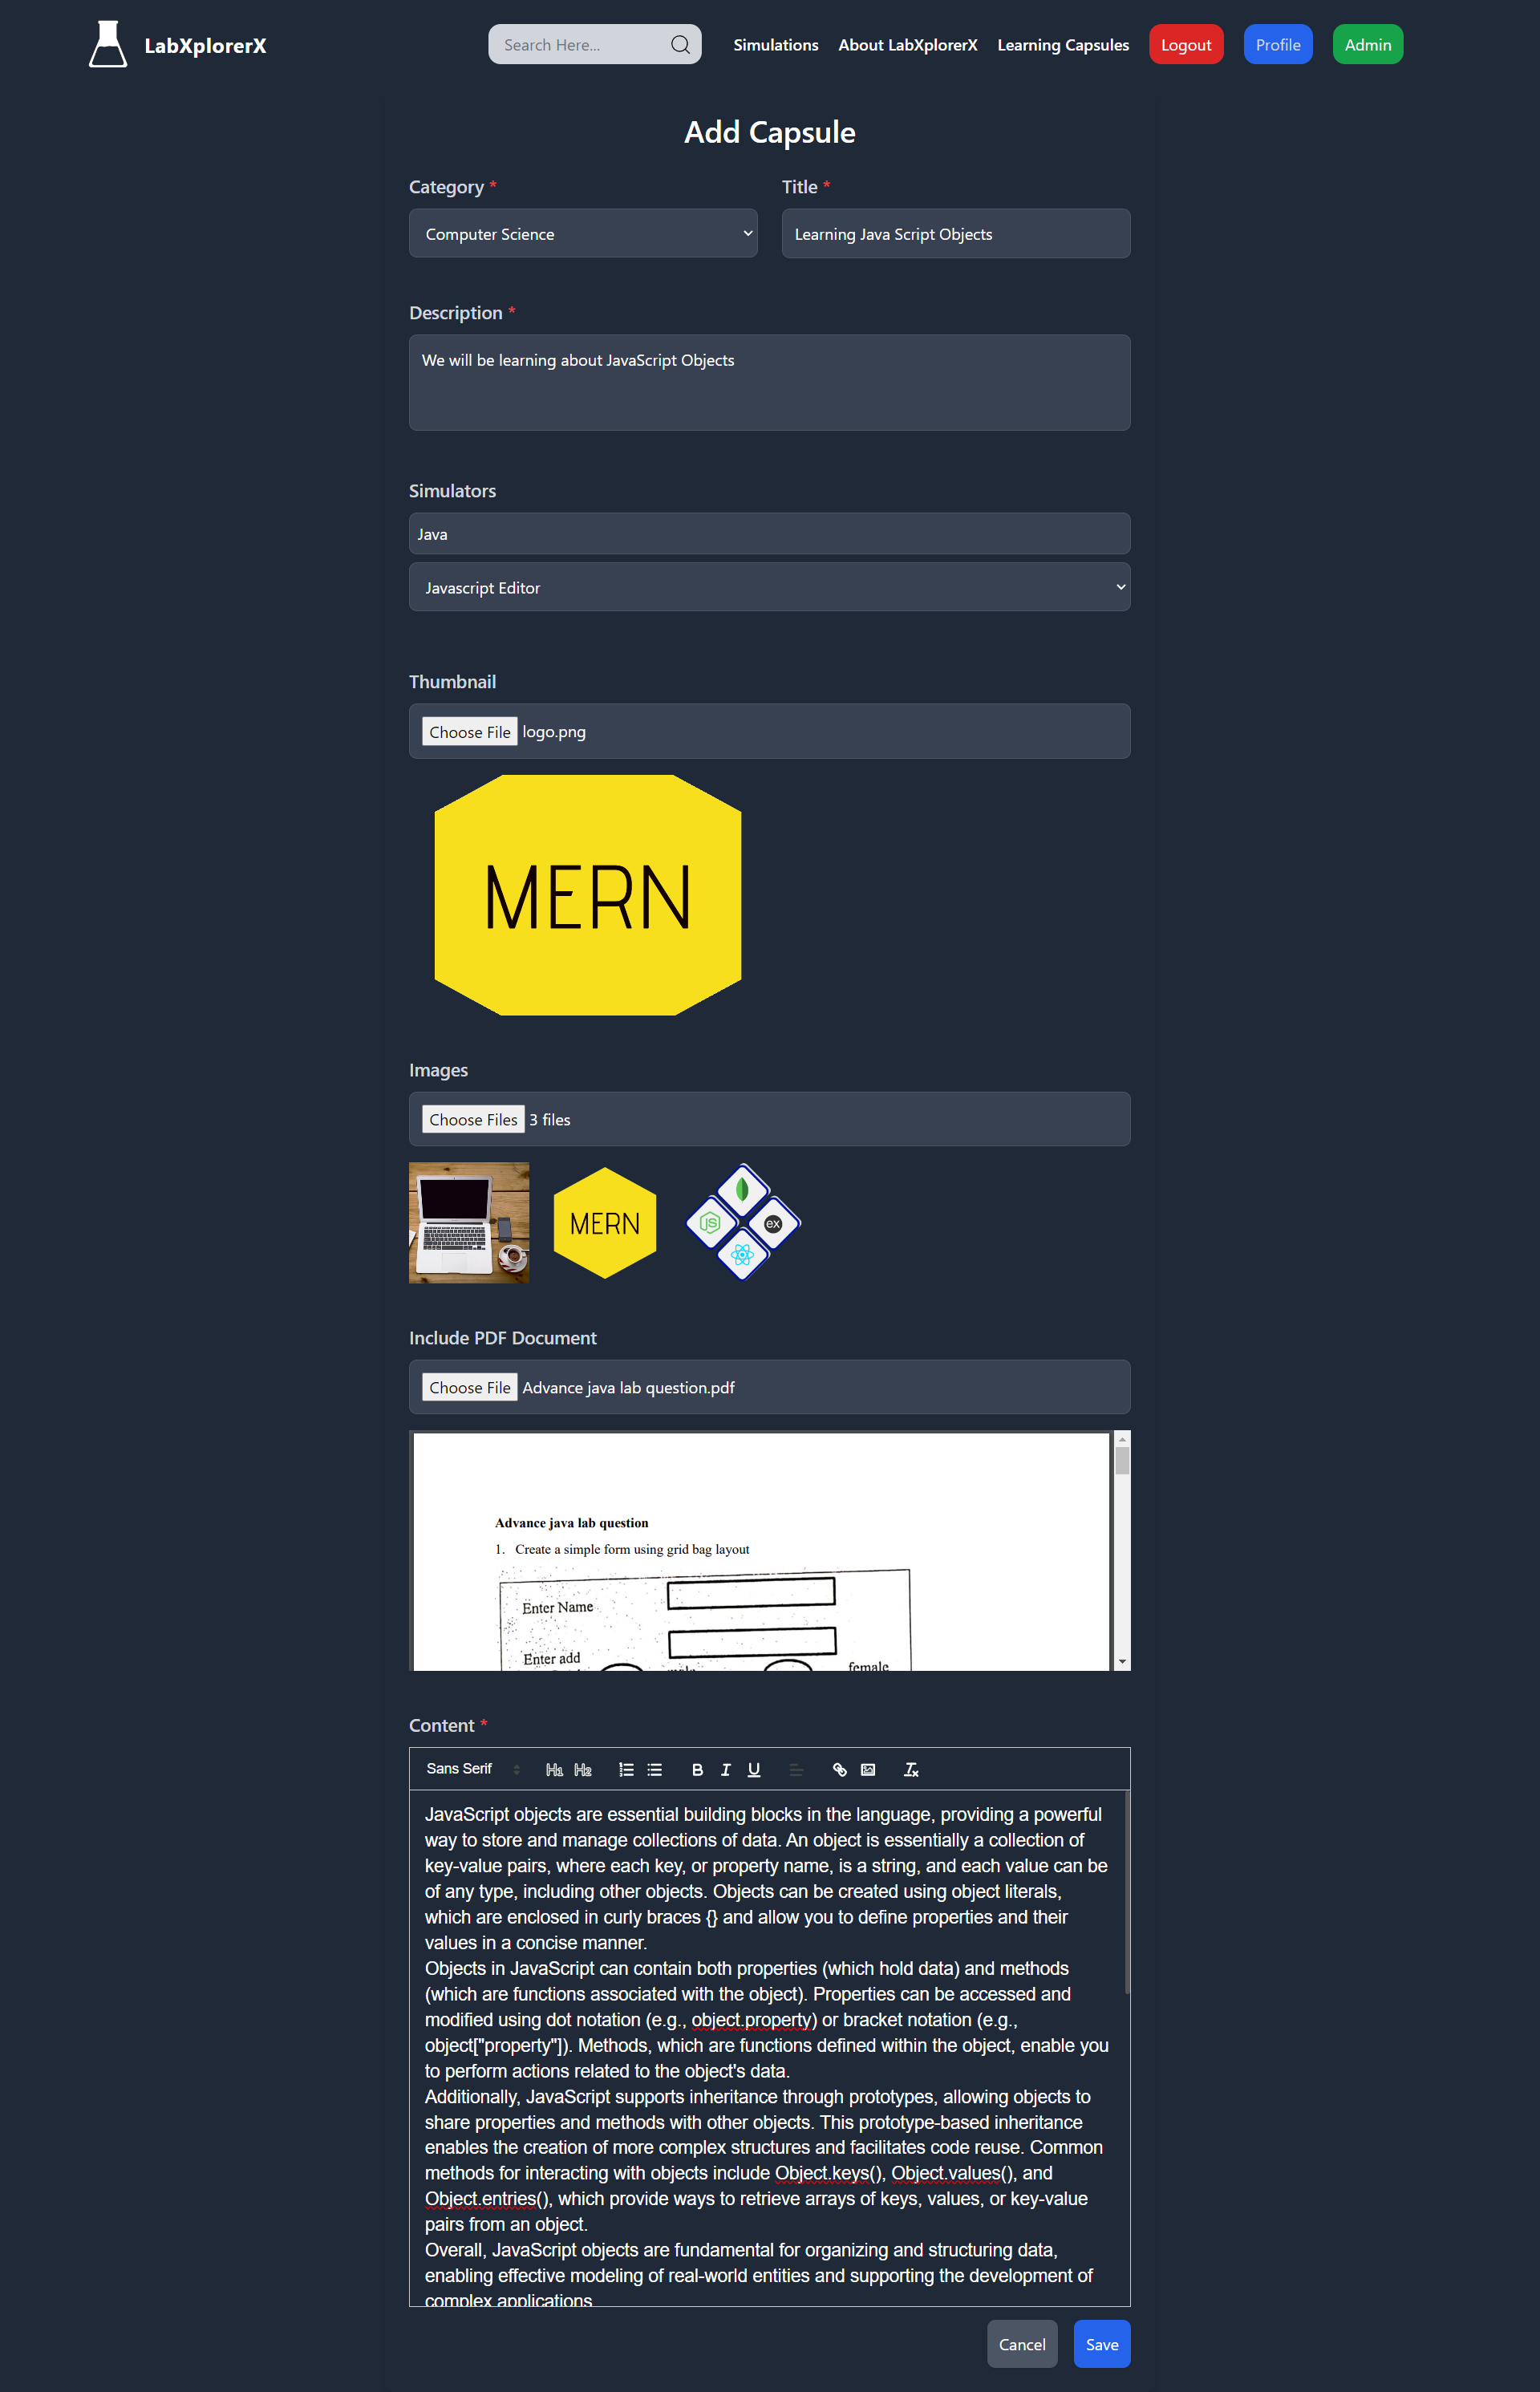
\includegraphics[width = 15cm]{Diagrams/output/addcapsule.png}
     \caption{Add Capsule}
 \end{figure}
 \begin{figure}[H]
    \centering
     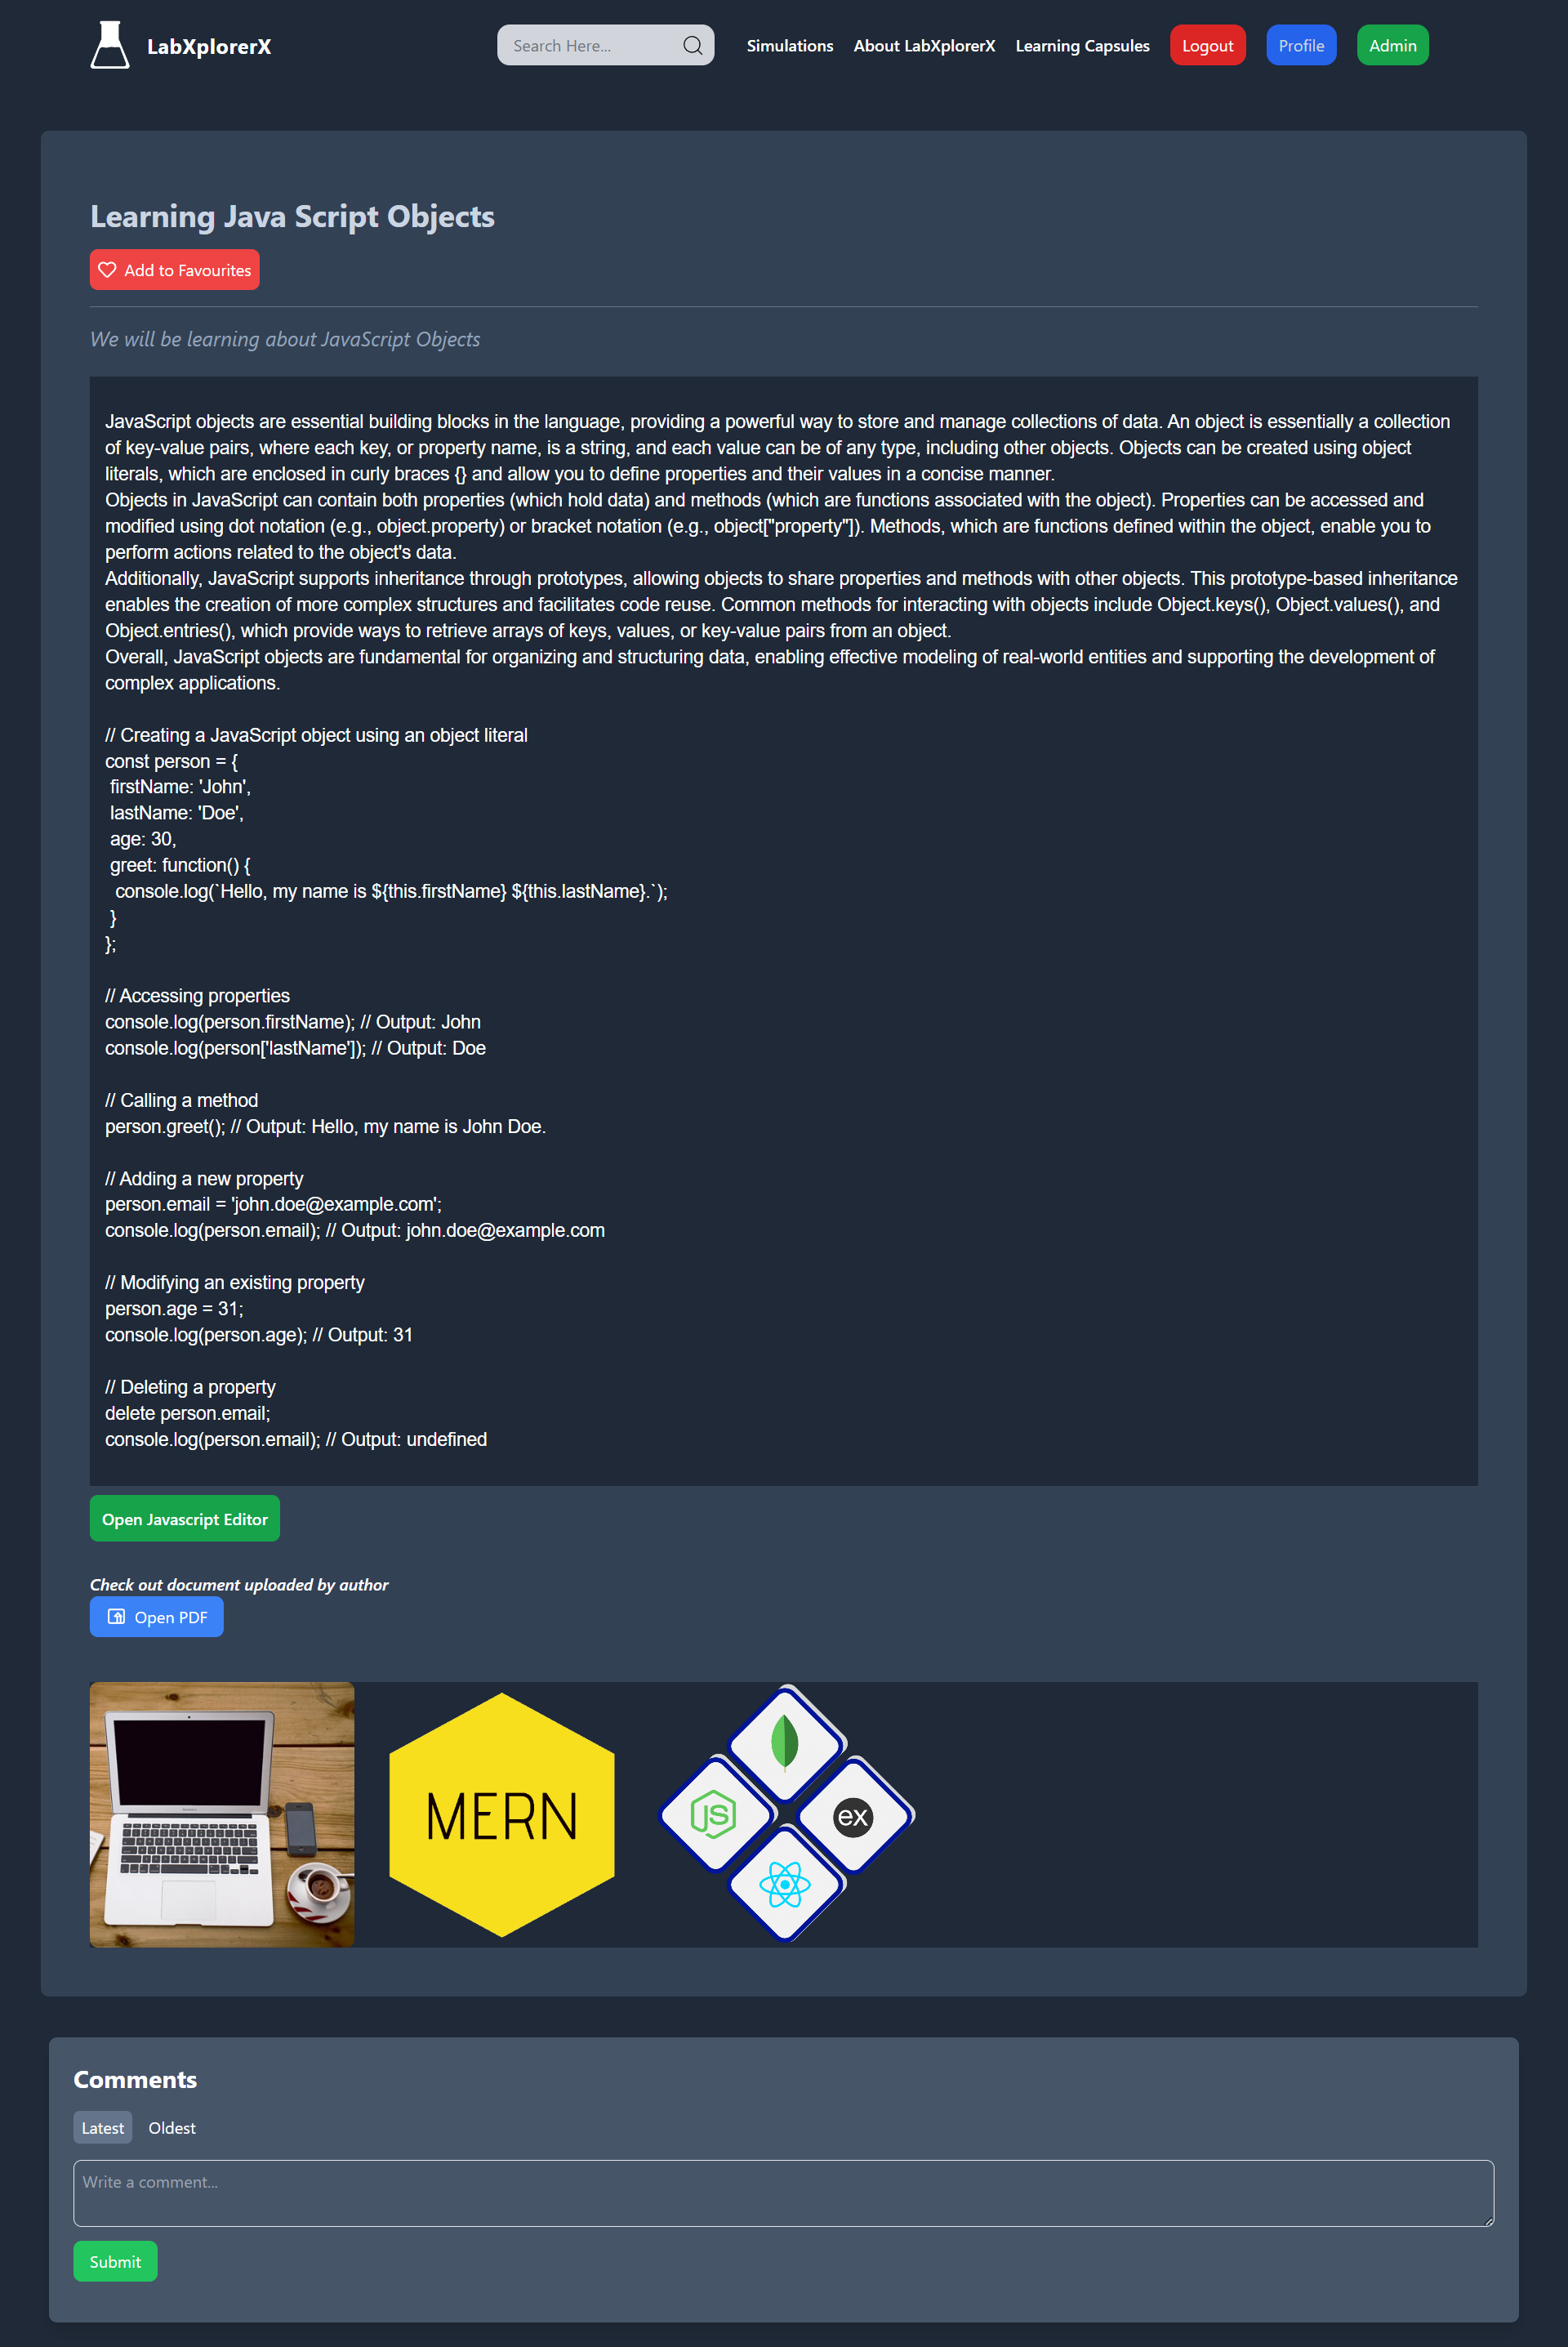
\includegraphics[width = 16cm]{Diagrams/output/after_addition.png}
     \caption{After Additon of Capsule}
 \end{figure}
\section{Work Remaining}
As the LabXplorerX project progresses, several key tasks remain to be completed. The development team will focus on creating additional simulations to further expand the interactive learning opportunities available to students. The implementation of user profiles is also pending, which will enable students to personalize their learning experience, track progress, and manage their accounts. Additionally, a discussion forum needs to be integrated into the platform, allowing students and teachers to engage in meaningful conversations, share ideas, and collaborate on learning activities.

\begin{itemize}[leftmargin=1cm]
    \item \textbf{More Simulations:} Continue creating additional simulations to broaden the range of interactive learning experiences available to students.
    
    \item \textbf{User Profiles:} Implement personalized user profiles, enabling students to track their progress, manage their accounts, and enhance their learning experience.
    
    \item \textbf{Discussion Forum:} Develop and integrate a discussion forum, facilitating communication and collaboration between students and teachers within the platform.
\end{itemize}